\documentclass{article}[12pt,a4paper]

\usepackage{enumitem}
\usepackage{graphicx}
\usepackage{parskip}
\usepackage{fancyhdr}
\usepackage{nopageno}
\usepackage{fontspec}
\usepackage{hyperref}
\usepackage{listings}
\usepackage{color}
\usepackage{courier}
\usepackage{fancyvrb}
\usepackage{subcaption}
\usepackage{longtable}

\hypersetup{
  colorlinks,
  citecolor=black,
  filecolor=black,
  linkcolor=black,
  urlcolor=black
}

\definecolor{codegreen}{rgb}{0,0.6,0}
\definecolor{codegray}{rgb}{0.5,0.5,0.5}
\definecolor{codepurple}{rgb}{0.58,0,0.82}
\definecolor{backcolour}{rgb}{0.95,0.95,0.92}
\definecolor{uigreen}{RGB}{82,170,94}
\definecolor{uiyellow}{RGB}{240,173,78}
\definecolor{uiblue}{RGB}{91,192,222}

\definecolor{specialblue}{RGB}{128,176,255}
\definecolor{specialorange}{RGB}{255,188,142}
\definecolor{specialturquoise}{RGB}{152,239,242}
\definecolor{specialred}{RGB}{249,119,117}
\definecolor{specialpurple}{RGB}{155,118,242}
\definecolor{specialyellow}{RGB}{244,216,112}
\definecolor{specialgreen}{RGB}{20,123,49}

\definecolor{lightgray}{rgb}{.9,.9,.9}
\definecolor{darkgray}{rgb}{.4,.4,.4}
\definecolor{purple}{rgb}{0.65, 0.12, 0.82}

\newfontfamily\dosis{Dosis-Bold}
\setmonofont{Office Code Pro}

\lstdefinelanguage{JavaScript}{
  keywords={typeof, let, const, new, true, false, catch, function, return, null, catch, switch, var, if, in, while, do, else, case, break, String, Number, Boolean, Object, Array, Date},
  keywordstyle=\color{blue}\bfseries,
  ndkeywords={class, export, boolean, throw, implements, import, this, default, from},
  ndkeywordstyle=\color{darkgray}\bfseries,
  identifierstyle=\color{black},
  sensitive=false,
  comment=[l]{//},
  morecomment=[s]{/*}{*/},
  commentstyle=\color{purple}\ttfamily,
  stringstyle=\color{red}\ttfamily,
  morestring=[b]',
  morestring=[b]"
}

\lstdefinelanguage{css}{
  morekeywords={accelerator,azimuth,background,background-attachment,
    background-color,background-image,background-position,
    background-position-x,background-position-y,background-repeat,
    behavior,border,border-bottom,border-bottom-color,
    border-bottom-style,border-bottom-width,border-collapse,
    border-color,border-left,border-left-color,border-left-style,
    border-left-width,border-right,border-right-color,
    border-right-style,border-right-width,border-spacing,
    border-style,border-top,border-top-color,border-top-style,
    border-top-width,border-width,bottom,caption-side,clear,
    clip,color,content,counter-increment,counter-reset,cue,
    cue-after,cue-before,cursor,direction,display,elevation,
    empty-cells,filter,float,font,font-family,font-size,
    font-size-adjust,font-stretch,font-style,font-variant,
    font-weight,height,ime-mode,include-source,
    layer-background-color,layer-background-image,layout-flow,
    layout-grid,layout-grid-char,layout-grid-char-spacing,
    layout-grid-line,layout-grid-mode,layout-grid-type,left,
    letter-spacing,line-break,line-height,list-style,
    list-style-image,list-style-position,list-style-type,margin,
    margin-bottom,margin-left,margin-right,margin-top,
    marker-offset,marks,max-height,max-width,min-height,
    min-width,-moz-binding,-moz-border-radius,
    -moz-border-radius-topleft,-moz-border-radius-topright,
    -moz-border-radius-bottomright,-moz-border-radius-bottomleft,
    -moz-border-top-colors,-moz-border-right-colors,
    -moz-border-bottom-colors,-moz-border-left-colors,-moz-opacity,
    -moz-outline,-moz-outline-color,-moz-outline-style,
    -moz-outline-width,-moz-user-focus,-moz-user-input,
    -moz-user-modify,-moz-user-select,orphans,outline,
    outline-color,outline-style,outline-width,overflow,
    overflow-X,overflow-Y,padding,padding-bottom,padding-left,
    padding-right,padding-top,page,page-break-after,
    page-break-before,page-break-inside,pause,pause-after,
    pause-before,pitch,pitch-range,play-during,position,quotes,
    -replace,richness,right,ruby-align,ruby-overhang,
    ruby-position,-set-link-source,size,speak,speak-header,
    speak-numeral,speak-punctuation,speech-rate,stress,
    scrollbar-arrow-color,scrollbar-base-color,
    scrollbar-dark-shadow-color,scrollbar-face-color,
    scrollbar-highlight-color,scrollbar-shadow-color,
    scrollbar-3d-light-color,scrollbar-track-color,table-layout,
    text-align,text-align-last,text-decoration,text-indent,
    text-justify,text-overflow,text-shadow,text-transform,
    text-autospace,text-kashida-space,text-underline-position,top,
    unicode-bidi,-use-link-source,vertical-align,visibility,
    voice-family,volume,white-space,widows,width,word-break,
    word-spacing,word-wrap,writing-mode,z-index,zoom},
  morestring=[s]{:}{;},
  sensitive,
  morecomment=[s]{/*}{*/}
}

\lstset{
   language=JavaScript,
   backgroundcolor=\color{backcolour},
   extendedchars=true,
   basicstyle=\footnotesize\ttfamily,
   showstringspaces=false,
   showspaces=false,
   numbers=left,
   numberstyle=\footnotesize,
   numbersep=9pt,
   tabsize=2,
   breaklines=true,
   showtabs=false,
   captionpos=b
}

\graphicspath{ {img/} }

\pagestyle{fancy}
\lhead{Porfiry Quiz Maker}
\lfoot{Daniel Roberts 4699}
\rfoot{Shrewsbury Sixth Form College 29285}
\rhead{Page \thepage}
\renewcommand{\headrulewidth}{0.4pt}
\renewcommand{\footrulewidth}{0.4pt}

\begin{document}

\title{WJEC GCE Computing CG4 - Extended Project}

\author{Candidate Name: Daniel Roberts\\
		Candidate Number: 4699\\
		Centre Name: Shrewsbury Sixth Form College\\
		Centre Number: 29285}

\date{}
\maketitle

\tableofcontents

\cleardoublepage

\part{Analysis of the Business} % (fold)
\label{prt:analysis_ _of_ _the_ _business_}
This initial part of the documentation features the analysis that was performed on the business. It includes the business' background, as well as an in-depth investigation on their current system, featuring document inspections, interviews, and observations. Also included is a problem definition, wherein the broad aims of the project are outlined; this definition also makes reference to the limitations of the solution. Finally, detailed objectives are clearly laid out, providing an overview of exactly what the solution should achieve.

% Import background
\section{Background}

\subsection{About the Business}

The Priory School is a medium sized secondary school located in Shrewsbury, Shropshire. The school is a founding member of the Salop Teaching Alliance, and employs over 100 teaching staff, with approximately 900 pupils on roll. Pupils range in age from 11 - 16, and each belongs to an individual form group. During it's previous two inspections, Ofsted judged the school to be Outstanding, the highest possible rating. Additionally, the school has the highest attendance rate in the county, and achieves exam results well above the national average. 

A change of leadership in January 2015 resulted in the previous headteacher, Ms Candy Garbett, leaving the school; Mr Michael Barratt, previously of Adams Grammar School, Newport, became the new principal. Following this change in leadership, the school has sought to embrace the advantages of technology, and has invested in several new systems, including an online homework tracker, a virtual learning environment, and a library tracking system. This newfound acceptance of technology opens the way for this project.

\subsubsection{A New Beginning?}
Due to Michael Barratt's previous experience in a grammar school, a number of additional changes have taken place, particularly relating to the management structure. Previously, each student belonged to a form group - one of Acton, Baxter, Clive, Houseman, Darwin or Webb. There were five of these houses throughout the school, one for each year - a 7A, 8A, 9A, 10A and 11A.

 Each year was controlled by a senior member of staff, usually one who had worked at the school for a large period of time; these were known as the \textit{head of year}. For example, the head of Year 7, Nick Bucknall, would be in charge of 7A, 7B, 7C, 7H, 7D and 7W, and would meet with the Year 7 form tutors each week, provide assemblies for Year 7, and so on. 

This horizontal approach has now been modified to a vertical one: each previous head of year is now known as a \textit{head of house}. Rather than controlling an individual year, they now control an individual house; for example, Nick Bucknall is now in charge of Acton, and so controls 7A, 8A, 9A, 10A and 11A.

\subsection{About the Project}
Like many schools, The Priory School makes use of a form time in the afternoon. During this process, students are registered, bulletins are read out, and a timetabled activity is carried out; these activities usually include silent reading, a group debate, and quizzes. These quizzes are usually designed by the head of year, and include a range of topics, from current affairs, educational matters, and simple trivia.

Currently, these quizzes are delivered to the forms on a Microsoft Word document, via the school's LAN. The members of the form work together to arrive at what they believe to be the correct answer, and once all questions have been answered, the form tutor marks the quiz and returns the result to the head of year, usually orally. Which would aid in following the school's new policy of ``togetherness''.

% Import investigation of the current system
\section{Investigation of the Current System}
This section details the in-depth investigation that was performed on the current quiz system used by the school. Initial contact with the school was made via an email to one Mr Nick Bucknall, currently head of Year 8, on the 30th June 2015. Following a brief email exchange, the details of which can be found below, Below can be found the different aspects that were investigated.

% \subsection{Overview of System}
% Currently, the school does not have a formal, standardised system in place. A somewhat ad-hoc approach is currently used, using a combination of emails, documents scattered across the network, and verbal communication. Obviously, this approach has a number of issues, the details of which can be found below in the observations performed, as well as the analysis of the current system's limitations.

\subsection{Interviews}
A number of interviews were held with staff at the school. Three form tutors were interviewed, in order to gain an insight into how they believe form times could be improved through the use of interactive quizzes, and to get an idea of how they would like such a system to work. Additionally, Nick Bucknall, a head of year at the school, was interviewed; he was chosen in order to gain information on what results the system should calculate, and how best to integrate such a system within the school. He was also chosen to get a further idea of the faults with the current system. Full transcripts for each of the interviews are included below.

\subsubsection{Bryan Warr}

\textit{\textbf{DR:}} So what would you say is the main focus of form time?

\textit{\textbf{BW:}} Okay. So, there's several different types of form time. One could be focusing the students on silent reading, one could be on numeracy, one could be on literacy, another could be on a discussion - on something moral or spiritual. Obviously we've got assembly time as well, but it also depends on the audience - it depends on whether they're Year 7 or whether they're Year 11. So for Year 7's it would be different to Year 11's. For example, Year 11's might spend time revising, or focusing on exam technique; but Year 7's, a lot of time is spent with Year 7's building up the relationship with their tutor. So some of that could be activities that get them all working together.

\textit{\textbf{DR:}} I see. How important is that during the later years?

\textit{\textbf{BW:}} Yeah, it's still important, definitely. I suppose it depends on whether your tutor is new or not - you might have a tutor who's newer to Year 10 or Year 11, and wants to spend their time getting to know them. If you've had a tutor that's taken you all the way through, like my tutor group, then you don't need those ice breakers as much - you know each other quite well.

\textit{\textbf{DR:}} And how often does it occur that form teachers leave halfway through?

\textit{\textbf{BW:}} Here it's not very often. It's not as often as it is in other schools - in some schools it's all the time. My last school, I took a group through Year 11, and it was unusual, because every single tutor in that year group was with them from Year 7 to Year 11, which is very rare. But here for example, our Year 10 tutor group, pretty much similar tutor team from the start to the end. There's been a little change - so tutors do change, but there's always a set activity list from the head of year, head of house I should say.

\textit{\textbf{DR:}} So does the head of year have more control than the individual form tutors?

\textit{\textbf{BW:}} Yes. The form tutor is told by the head of year, well next year it will be the head of house, what to do. So we get given a timetable, it's on the wall, we get given a tutor program. Do you wanna see one?

\textit{\textbf{DR:}} Yeah, that would be helpful.

\begin{center}
\textit{\textbf{* DR and BW move to the classroom wall, to look at the timetable *}}
\end{center}

\textit{\textbf{BW:}} So these change every year. This is the Year 10 one - this is the summer one.

\begin{center}
\textit{\textbf{* Microphone fails to pick up conversation for the next 30 seconds. BW prints out tutor timetables for Year 9, Year 10 and Year 11, available below. BW and DR sit back down again. *}}\\
\end{center}

\textit{\textbf{BW:}} So you'll see that that one's key stage 3, and then you've got Year 10 and Year 11. So is you're idea maybe that you'd trial it here, or were you thinking...?

\textit{\textbf{DR:}} Yeah. The thing we've got to do is think of an idea for a system, and then go to a business - in my case it's here - and do interviews, with people who would use the system; hand out questionnaires, and perform observations. I've done my observation because I just used my experience here, and I'm doing interviews now.

\textit{\textbf{BW:}} So, Mr Bucknall would be a good one to talk to.

\textit{\textbf{DR:}} I've arranged one with him.

\textit{\textbf{BW:}} He's a head of house next year. So he's obviously, he's directly - he writes that. So the tutors, heads of house, who else? Also SLT, any members of SLT - I'm on SLT next year as well. Obviously the assemblies are run by members of SLT, but you can see there's a theme running through them - Year 9, you've got literacy, numeracy, in each one; you've got group discussions or activities, you've got silent reading in each one, because it just needs to be established. In Year 11, that would be revision, or personal study. And in Year 10 we give them that opportunity as well - we say, ``right, if you want to study, you do that.'' It's a lot more open than in Year 7.

\textit{\textbf{DR:}} The idea I had focuses mainly on the quiz aspect - automating it, so to speak, and making it more competitive. How do you feel about quizzes? I can see they're fairly regular on the timetable, but less so in Year 11.

\textit{\textbf{BW:}} Well, Miss Mitchell used to do them, and she was quite good at them. The quizzes are...I find them a bit hit and miss, on my own quizzes. The Year 10's do like them, my Year 10's. If they were automated, that would work. And if it was a competition between houses...

\textit{\textbf{DR:}} Yes, that's what I was thinking.

\textit{\textbf{BW:}} That's what we're...that would be really...I would have thought that would be quite well received, because obviously we're moving towards bigging up the house system next year. 

\textit{\textbf{DR:}} Okay.

\textit{\textbf{BW:}} So the house system is going to be more prevalent, so the fact that you're competing into forms...and also, heads of house would like it, because you've halved their workload, if a quiz is being laid on every week, definitely would be useful. It's obviously going to be difficult that you've got 7, 8, 9, 10 and 11...

\textit{\textbf{DR:}} All of whom need doing.

\textit{\textbf{BW:}} With different quizzes. That wouldn't be too difficult.

\textit{\textbf{DR:}} No. So, when I was in Year 11, Mr Bucknall seemed to control the quiz system quite heavily.

\textit{\textbf{BW:}} Yep.

\textit{\textbf{DR:}} So he'd make the quiz himself.

\textit{\textbf{BW:}} Yes, that's right.

\textit{\textbf{DR:}} And then handed out different quizzes. How do you feel about that, if that's what Mrs Shaw does with you?

\textit{\textbf{BW:}} Happy with that. If it was centralised, it would be even easier. So if the heads of house didn't have to handle that, if it was in a central system, that you could access, that would be easier.

\textit{\textbf{DR:}} So say there was an icon on the desktop, that opens up the program, showing the quiz for the week. 

\textit{\textbf{BW:}} Yes. Perfect. And if you chose Year 7, with a choice of the year groups, that would be easy. So the tutor could say ``right, I want the Year 7 one to come up'', that would be perfect. Yeah.

\textit{\textbf{DR:}} Because what I was thinking was the different heads of year, or houses now...if they wanted a quiz, they'd write it using the system, and then they'd have access to their form groups, so then they could target...and then they could send it that way. Would that be something they'd be interested in?

\textit{\textbf{BW:}} Possibly, but don't forget that now they're heads of house...so Mr Bucknall, who's got Darwin, he's now got five years. So again it's the same issue, each head of house has got to make lots of quizzes. 

\textit{\textbf{DR:}} So, there aren't heads of year anymore, there are houses?

\textit{\textbf{BW:}} Right. So we've got Acton, Baxter, Clive, Darwin, Houseman and Webb; and then each one's a house with a vertical setup to it.

\textit{\textbf{DR:}} I see.

\textit{\textbf{BW:}} So you're going to have the same issue with each one, in that they've got to differentiate between the years. And what they wouldn't want to do is replicate their work. So I don't think they'd be happy if they were...say Mrs Smith was doing this, and she had to do all the years, and Mrs Heath had to do the same, that would be a lot of repetition, whereas we could probably do the same...you could do the same thing for each one, couldn't you? If you did Year 7, just...bam. Year 8...right, just like that. That would be more sensible.

\textit{\textbf{DR:}} Okay. So, with assemblies and such, are the heads of houses taking each individual house each week? It wouldn't be say Mr Bucknall who speaks to the whole of Year 11 on a Tuesday?

\textit{\textbf{BW:}} Occasionally there will be a need for us to speak to Year 11 or Year 10 to do with certain aspects. But the majority of assemblies are with the houses, so it would be Mr Bucknall talking with Darwin - all the years. Okay? So it will be a house assembly. And we have whole school assemblies now on Mondays, first Monday of the month, which Mr Barratt does. So that's every Monday, and it's whole school, in the sports hall.

\textit{\textbf{DR:}} Kind of like it was at the end of term before?

\textit{\textbf{BW:}} Exactly, yeah, yeah. He's got it every month now, so we get together as a whole.

\textit{\textbf{DR:}} Right. So how do you feel...if the school's looking to improve cooperation between houses, how would you feel about that taking place in form time?

\textit{\textbf{BW:}} How do you mean?

\textit{\textbf{DR:}} Well, if, say, there was the quiz, say on that side of the screen, and on the other side was a view showing how the other forms are doing, in real time, would that be something you'd be interested in?

\textit{\textbf{BW:}} It could be interesting, yeah. Could be interesting. Definitely brings in the element of competition, live, rather...

\textit{\textbf{DR:}} Yeah, because that makes it a lot more interesting, than finding out say a week after that Baxter has won.

\textit{\textbf{BW:}} The only problem you've got is that they wouldn't necessarily be the same years on the same days.

\textit{\textbf{DR:}} How do you mean?

\textit{\textbf{BW:}} Well you'll have Acton...you're Year 7 quiz could be on the same day, but Year 7 and Year 10 might not be. Because the tutor programs are different, because they have to be, because of the assemblies and rooms, so for example the KS4 assembly there is on a Tuesday, but there it's silent reading. So they could be doing a quiz, but these lot could be in assembly. So there could be a house assembly on, when you've got Acton doing it. So, you'd have to look...

\textit{\textbf{DR:}} But horizontally, that wouldn't be an issue.

\textit{\textbf{BW:}} Right, horizontally, it would work, yeah. All of Year 7 would be together at the same time, unless there's a house assembly - if there's a house assembly on, it means that house would be out. So you'd have to look for where there's that literacy or numeracy activity, or something like a silent reading activity, where there's something with a group discussion. But I'm sure the heads of house wouldn't mind if, once a month, one of those...you'd have to ask Mr Bucknall of course, I'm sure he wouldn't mind...if one of those was taken up with a house quiz. Because if you did that, I'm just thinking...within a half term, you could get one quiz in for every year group. You could take one silent reading or one literacy or numeracy activity, and replace that with a house quiz, for the year group, that would work.

\textit{\textbf{DR:}} Okay. And what sort of topics would the quizzes best fit? Because when I did them, it kind of varied each week, so sometimes it would be culture, sometimes it would be general...stuff.

\textit{\textbf{BW:}} General knowledge is always good. Music's always good. Popular culture. Anything like that you could have. You could make it so they were subject related. So you could have history, geography or maths.

\textit{\textbf{DR:}} Right. So how would you, as head of maths, feel about there being a maths quiz?

\textit{\textbf{BW:}} Yeah. I'm happy with that. We're doing inter-house competitions within the subject, so we're going to do a Countdown activity. But I'd be absolutely fine with that, a maths quiz now and again, because again, it raises maths in the school. I'm sure the other heads of department are the same.

\textit{\textbf{DR:}} Okay. Trouble is trying to make it seem like a quiz, rather than a test, which I guess it would be.

\textit{\textbf{BW:}} Exactly. And also, you've gotta be careful with differentiation, because some students are much better at maths than others.

\textit{\textbf{DR:}} So would the top group have done things that the lower groups would have done?

\textit{\textbf{BW:}} Yes. Yeah, they'd have done some different things, so...maths quiz. See, my tutor group's a good example. I've got a tutor group where I've got some brilliant mathematicians, and some who really struggle, and to give them maths quizzes is always difficult, because some are at an advantage straight away - even with Countdown they're at an advantage. That would be a tricky one. General knowledge is probably better because everyone can access that. I mean, even if you did a History quiz, some people would be at an advantage. That's a tricky one. You could make it so that it would be subject related quiz, on a one off, where there was bits of Maths, bits of History. I suppose you could do that, make it more general.

\textit{\textbf{DR:}} Yeah, cause each form has people who are good at some things...

\textit{\textbf{BW:}} That might make it more accessible.

\textit{\textbf{DR:}} And how well would it work? If the form had to work with one another, to work out the answer?

\textit{\textbf{BW:}} That would be fine. Yeah, it wouldn't be an issue. The forms are used to working together.

\textit{\textbf{DR:}} And are all forms going to be happy working that way? Certain forms and year groups, I imagine, are less likely to work well with that sort of system.

\textit{\textbf{BW:}} Depends on the form tutor really. But the majority of the time, the form tutors accept what's asked of them. Certainly the majority of cases.

\textit{\textbf{DR:}} And how would participation be dealt with? There'd be some people at the back of the room who don't participate.

\textit{\textbf{BW:}} Right. You could do...to ensure participation, could be something like use the iPads. You could do something either...we do work using Socrative, using that. It's an app where everybody has to answer. So, I set the Socrative quiz up recently with my Year 7's. It's a web based one, so something like this would work. So with Socrative, I set a quiz up for the Year 7's, and you can see the live results come in. What they do is they can login to your room, and the quiz comes up as you're doing it - you get live results, with a load of reports. So I've got these results here, and these have all come through, and that's how it comes through. So there's the questions and answers - I can see that who's answered, and as they were doing it, I knew that Izzy hadn't done it. So maybe something like that would ensure participation.

\textit{\textbf{DR:}} So this is kind of like the old Quizdom system they used in Science.

\textit{\textbf{BW:}} Quizdom, exactly.

\textit{\textbf{DR:}} I never thought that worked very well.
 
\textit{\textbf{BW:}} No, these work a lot better - there's less faffing about. It's a web based system, so the room is accessible to anyone - it's constant; that will always be my room, whatever quiz I do. But that would work. Other than that, you're sort of relying on the teacher just...getting everybody involved.

\textit{\textbf{DR:}} Is that something the school is looking at - raising participation - or is that not really an issue?

\textit{\textbf{BW:}} We're looking at raising participation with the house system, and anything that does that is going to be useful. I don't think engagement in general is a problem in this school.

\textit{\textbf{DR:}} So if this sort of system were implemented in form time - purely in form time - would that be an issue, or should it be expanded for use in subjects?

\textit{\textbf{BW:}} I think it would be useful in form times to start with. Purely to address the problem the heads of house have. It also makes it more unilateral, doesn't it? Yeah, I think that would work.

\textit{\textbf{DR:}} How technical would you say that you are?

\textit{\textbf{BW:}} I'm pretty good. No, I'm not too bad. I can deal with most things, but not everybody's the same.

\textit{\textbf{DR:}} No. I'm trying to make it as simple as possible - thinking of people like Mrs England.

\textit{\textbf{BW:}} Yeah, some people would struggle. So it literally needs to be...two clicks. One click to get into the program, click to choose your year, maybe another to start the quiz.

\textit{\textbf{DR:}} How would you feel about a login system, where you had to sign in?

\textit{\textbf{BW:}} A login system would be fine. It would prevent the students hacking it.

\textit{\textbf{DR:}} Yeah, that's what I'm thinking.

\textit{\textbf{BW:}} Yeah, that would work. We're used to logging in to stuff. So yeah, happy with that.

\textit{\textbf{DR:}} This sounds a little crude, but would you be tempted to help your form in any with, if there was a reward for the best performing house?

\textit{\textbf{BW:}} Right. Are you suggesting would I cheat?

\textit{\textbf{DR:}} Yes.

\textit{\textbf{BW:}} Right. No, it's a good question. No, I wouldn't help them with it. I don't think they'd need my help - they work quite well together. I'm not convinced that every teacher would feel the same. \textit{\textbf{*laughs*}}

\textit{\textbf{DR:}} Okay. And is that going to be different depending on their year group?

\textit{\textbf{BW:}} Possibly, yeah. For Year 7 we'd approach it differently to Year 11.

\textit{\textbf{DR:}} And how suitable would this be if the school had, say, a theme of the term or theme of the week?

\textit{\textbf{BW:}} They do come up, but they would be more weekly things - so sometimes you have Anti-Bullying Week, or Global Entrepreneurship Week - so they come up now and again.

\textit{\textbf{DR:}} I see. And would this system come in useful for the quiz aspect of that?

\textit{\textbf{BW:}} Yeah, absolutely. And I'll tell you who else would be interested in this as well: Mrs Hancox and Miss Morris who run Life. Life would be really interested in this. I'm just thinking outside the box, purely because Friday lesson 2, when you have Life, you would have all of the year group in the same lesson at the same time - everybody in the school. So there might be an opportunity in Life as well.

\textit{\textbf{DR:}} I'll send them an email I think, thank you.

\textit{\textbf{BW:}} That might be worth talking about. You know...did Miss Hancox or Miss Morris teach you?

\textit{\textbf{DR:}} Miss Morris taught me for three years, yes.

\textit{\textbf{BW:}} Right, so you know her. So they're the heads of Life - they'd be interested in this, and that would be a good opportunity to use it, potentially. And with Life, they've got all sorts of things, so there's a lot of opportunity for quizzes.

\textit{\textbf{DR:}} If this were rolled out, how likely is it that it were actually used?

\textit{\textbf{BW:}} I think if people are told to use it, they'll use it.

\textit{\textbf{DR:}} Okay. And how would the heads of house tell you?

\textit{\textbf{BW:}} When I get this from Mrs Shaw, I follow that, because she tells me to. We know what we have to do - this on a Monday, that on a Wednesday. It might not be that we do the same thing, but we do some literacy and numeracy, then we do a group discussion or quiz, and then we have assembly. So we have that programme, and we follow it. We're actually checked up on whether we do that. SLT will check, randomly - we don't know when they're coming, but it's with the head of house, and they check what you're doing. If you're not doing what you're meant to...trouble.

\textit{\textbf{DR:}} Right. I remember last year, I had Mr Massey. And he wasn't...

\textit{\textbf{BW:}} \textit{\textbf{*laughs*}} You don't have to say any more!

\textit{\textbf{DR:}} And that was an issue sometimes.

\textit{\textbf{BW:}} Yeah. Okay. I feel your pain. \textit{\textbf{*laughs*}}

\textit{\textbf{DR:}} So, how would you feel about the quiz...

\textit{\textbf{BW:}} \textit{\textbf{*laughs*}}

\textit{\textbf{DR:}} About the quiz...\textit{\textbf{*laughs*}}...not starting until all the teachers had signed on?

\textit{\textbf{BW:}} Yeah, happy with that. I mean, it could be that you could trial it with one year group. You could ask the heads of house which year groups they feel most confident about giving it to. It might be that you've got a team of tutors in that year group who know they kids better, who've been together longer, who are maybe more confident dealing with this stuff, before you roll it out. Don't forget, you've got Year 7 tutors coming in September, who are gonna have to get to know their tutor groups. That'll be the priority for them. Year 11, pretty much starting them on exam technique...well, with the exception of your tutor \textit{\textbf{*laughs*}}. You want to get the ball rolling and get them into exam mode, so maybe a Year 9 team...\textit{\textbf{*laughs*}} yeah.

\textit{\textbf{DR:}} Sorry. \textit{\textbf{*laughs*}}

\textit{\textbf{BW:}} I dread to think! \textit{\textbf{*laughs*}} Who was in your tutor group? Name me some interesting characters.

\textit{\textbf{DR:}} Nick Porter.

\textit{\textbf{BW:}} Jesus. Right. Go on.

\textit{\textbf{DR:}} Doug Coull.

\textit{\textbf{BW:}} Oh right, not too bad.

\textit{\textbf{DR:}} Liam Davies.

\textit{\textbf{BW:}} \textit{\textbf{*laughs*}} Say no more - we're there!

\textit{\textbf{DR:}} \textit{\textbf{*laughs*}} So how would you feel about an email in the morning, reminding you of the quiz? Obviously you've got the timetable, but not all teachers are going to follow that.

\textit{\textbf{BW:}} \textit{\textbf{*laughs*}} Yeah, emails would work. Most of the teachers check their email in the morning.

\textit{\textbf{DR:}} That wouldn't be seen as too overbearing?

\textit{\textbf{BW:}} No, I don't think so. You could also set up a reminder on Outlook - that would work. Rather than an email, we could get a reminder, at whatever time the quiz is supposed to take place, so my Outlook is linked to my calendar. I get a reminder and it would just say ``Year 10 quiz - 1:40pm''. That might work as well.

\textit{\textbf{DR:}} Well, I think that's pretty much it.

\textit{\textbf{BW:}} Okay.

\textit{\textbf{DR:}} But thank you very much, you've been very helpful.

\textit{\textbf{BW:}} Anytime! I would set up a discussion with the heads of house - certainly Mr Bucknall.

\subsubsection{Wendy Blower}

\textit{Interview scheduled for 7th July.}

\subsubsection{Carla Hancox and Rachel Morris}

\subsubsection{Nick Bucknall}

\textit{Interview scheduled for 14th July.}

\subsubsection{Tim Goodman}

\subsection{Questionnaires}
An online questionnaire was created for students of the school to fill in, detailing their opinion on form times, how it could be improved through the use of quizzes.

\subsubsection{Questions}
The following questions were included	 on the questionnaire, distributed to students at the school:

\noindent\fbox{%
    \parbox{\textwidth}{%
        \begin{enumerate}[leftmargin=0cm,itemindent=.5cm,labelwidth=\itemindent,labelsep=0cm,align=left]
					\item How satisfied are you with your current form time experience? 1 2 3 4\\
					\item ``My form times are always well structured.'' How far do you agree or disagree with this statement? 1 2 3 4 5\\
					\item Out of the following activities you selected, which do you enjoy the most?
								\begin{itemize}
									\item Silent reading
									\item Knowledge quiz
									\item Group discussion
									\item Board games
									\item Physical activities
									\item Other\\
								\end{itemize}
					\item Approximately how often do quizzes feature in your form times? 1 2 3 4\\
					\item ``My form times would be improved if we did quizzes more often.'' How far do you agree or disagree with this statement? 1 2 3 4\\
					\item ``I find that quizzes improve the relationship between me and the rest of my form'' How far do you agree or disagree with this statement? 1 2 3 4\\
					\item Which topics have you been given quizzes on? Select all that apply.
								\begin{itemize}
									\item General knowledge
									\item Media
									\item Sports
									\item History
									\item Literature
									\item Relationships
									\item Brainteasers
									\item Other\\
								\end{itemize}
					\item To what extent do you interact with other forms in your year during form time? 1 2 3 4\\
					\item Do you believe form times would be improved by interaction with other forms? Yes No\\
					\item If you wish, please expand on your answer to the previous question.
				\end{enumerate}
    }%
}

\subsubsection{Results}
The following results were collected after the quiz had been live for 10 days. They were automatically generated using the 

\subsection{Observations}
Having been a member of the school community for over five years, I am well placed to provide an observation on how the school currently goes about creating, setting and analysing quizzes used in form times. Currently, no formal system is in place; an ad-hoc system is used, following this general pattern:

\begin{enumerate}
	\item The head of year creating the quiz thinks of a set of questions and possible answers, usually following a theme, and then writes them down on a Microsoft Word document. The correct answer is marked out, to aid the form tutor in marking the quiz. This document is then saved to a drive on the school's LAN.

	\item The head of year then notifies the individual form tutors of the quiz, usually at one of their weekly meetings, and tells them to conduct the quiz with their form group on a certain date.

	\item When the date is reached, the form tutor opens the document from the network, ensuring that the document is kept hidden to avoid members of the form viewing the correct answers.

	\item The form tutor reads each question out in turn, and the members of the form work together to attempt to work out the answer. They either come up with their own answer or choose from a list of options, depending on whether or not the question is multiple choice. The form tutor marks down the answer they chose, and this process repeats until the quiz is completed.

	\item Once all the questions have been answered, the form tutor adds up the total number of marks achieved by the form.

	\item The form tutor then passes the mark onto the head of year, either by email or when passing them in the corridor or the staffroom. This task is sometimes performed by a member of the form themselves, occasionally with the expectation that the mark achieved will be exaggerated somewhat.

	\item After receiving all the results, the head of year works out which form achieved the highest result, and which the lowest. This result is reported back to the year in the weekly assembly, often with a small reward for the highest achieving form.
\end{enumerate}

\subsection{Document Inspections}

\subsection{Similar Systems}
There are a number of systems available, both free and at a cost, that would allow the school to improve their current method of quiztribution (\textit{quiz distribution}). Several popular options are outlined below.

\subsubsection{Quiz Creation Websites}
A number of websites exist that allow users to design, play and share their own quizzes. These websites, including \textit{QuizWorks}, \textit{ExamTime} and \textit{QuizBean} generally follow the same pattern: the user creates an account, is directed to an interface wherein they can design a quiz, and is then given a link with which they can share the quiz with others. For basic quiz creation, these websites are free, though for more advanced usage (\textit{QuizWorks} defines an ``advanced'' quiz as one containing more than 15 questions), paid plans are available.

As these systems are websites, they can be accessed from practically any computer or mobile device, as long as there is an internet connection in range. This means that users can continue to work on their quizzes, whether designing or answering them, outside of their place of work.

Though these systems are undoubtedly useful, and could, with a few compromises, be easily integrated into the school's routines, they lack an awareness of the structure of a school. There is no concept of ``form groups'' or ``heads of year'', both are which are vital concepts if the system is to meet what the school desires. Additionally, they lack the ability to display a detailed analysis of the results (at least, not without paying a somewhat exorbitant fee - \pounds60 per month in the case of \textit{QuizWorks}), a side effect of their focus on individuals as opposed to groups.

\subsubsection{Quiz Creation Software Packages}
Similar to quiz creation websites, quiz creation software packages allow the user to design and play a quiz. However, these systems are desktop applications (the majority are designed for Microsoft Windows), and so can only be accessed from a single desktop or laptop system. Examples of these systems include \textit{Wondershare Quiz Creator}, \textit{Tanida QuizBuilder}, and \textit{Articulate Storyline 2}. Unlike the mostly free websites, these software packages are often very expensive: the three systems mentioned range in price from \$99 - \$1846 for a single license, with additional licenses costing even more.

To compensate for the high prices, these desktop applications contain a vast feature set. Quizzes of every imaginable type can be created, from drag-and-drop, multiple choice, word bank quizzes, and many more. Images can be included, points assigned, and complex animations can be set to make the quiz as visually appealing as possible. In addition, reports can be generated with tremendous amounts of data, showcasing practically every data point imaginable.

Useful though these features are, they are a touch overkill for what the school's purposes. The systems are not the easiest things to use in the world, something that, considering the teacher's relative lack of IT skills, is quite a drawback. Additionally, the high costs make the systems prohibitively expensive, considering the school's status as the worst funded school in the county.

\subsubsection{Quizdom}


\subsection{Justification of Methods}

\subsection{IPSO Chart}
This IPSO chart describes the inputs, outputs, storage locations and general processes that are associated with the system.

\begin{table}[h]
\centering
\begin{tabular}{|l|l|}
\hline
\multicolumn{1}{|c|}{{\bf Inputs}}                                                                                                                              & \multicolumn{1}{c|}{{\bf Processes}}                                                                                                                                                                                                                                                                         \\ \hline
\begin{tabular}[c]{@{}l@{}}Full name\\ Password\\ \\ Form name\\ \\ Quiz title\\ Quiz questions\\ Quiz answers\\ Forms the quiz should be sent to.\end{tabular} & \begin{tabular}[c]{@{}l@{}}Create HOY accounts from inputs\\ Create form group accounts\\ \\ Create and store quizzes\\ \\ Allow quizzes to be answered by\\ forms and store answers.\\ \\ Prevent quizzes from starting unless\\ all forms have joined.\\ \\ Mark quizzes and analyse results.\end{tabular} \\ \hline
\multicolumn{1}{|c|}{{\bf Storage}}                                                                                                                             & \multicolumn{1}{c|}{{\bf Outputs}}                                                                                                                                                                                                                                                                           \\ \hline
\begin{tabular}[c]{@{}l@{}}Store user accounts\\ Store individual quizzes with answers.\\ Store mark for quizzes.\\ Store analysis of results.\end{tabular}     & \begin{tabular}[c]{@{}l@{}}Quiz containing questions and answers.\\ Analysis of quiz results.\end{tabular}                                                                                                                                                                                                   \\ \hline
\end{tabular}
\caption{IPSO Chart}
\label{my-label}
\end{table}

\subsection{Limitations of Current System}
There are evidently a large number of issues with the above method. Firstly, distributing the quizzes via a word-processed document is not a particularly efficient method. It results in the network drive being cluttered with a variety of documents, perhaps with a non-existent naming scheme. This makes it harder for the form tutors to find the correct quiz for the week, slowing the whole process down. A more effective solution would be to have everything in it's own self contained system, with its own dedicated quiz screen, which points out the correct quiz to the tutors.

Additionally, having the questions and possible answers on the same document puts the integrity of the quiz at risk. Currently, form tutors get around this by hiding the document, but this can cause complications where students forget the possible answers, as well as other issues. It word be far more effective to always have the quiz displayed on screen on the interactive whiteboard, but the current system prohibits this.

Often, teachers forget about the quiz altogether, or believe it to be on a different date than when it is actually scheduled. This is a relatively common occurrence, and means that the quiz either has to be rescheduled (which those tutors who did remember find annoying), or that particular form has to miss out on the quiz that week; this can damage their overall reputation in the school community. A dedicated system could provide them a notification, perhaps via an email, that they should hold the quiz that afternoon. Additionally, the system could be set up in such a way that the quiz only begins once all the appropriate forms have connected.

Furthermore, the current system is not particularly fair. Students can spend as long as they wish on a single question, as long as the quiz is completed within the 25 minutes given to the form time. It would be fairer if the form was given a time limit of, say 60 seconds, after which the system automatically moves on to the next quiz.

The current system is also very isolated. Following the appointment of the new principal, the school has sought to implement the principle of ``togetherness'', whereby students work together more often. Though the current quiz system aligns itself with this philosophy to a degree (each form works together to come up with the answer), it could be improved by allowing a degree of interoperability between the forms. For example, if a quiz was being answered by all the forms in Year 8, one form could be given the opportunity to pose a question to the other forms, perhaps referencing one of the jokes sanctioned by the school.

By allowing the form tutors themselves to mark the quiz, their is a large risk of
inaccurate results being reported back, possibly altered in such a way that favours the form. Though this allows the head of year to display trust to his team of form tutors, there exists in the school a very competitive atmosphere, increasing the chance that such malpractice will occur. A safer approach would be to allow the system to mark the form's answers, and then report this directly to the head of year.

Though the heads of year throughout the school possess many fine and admirable qualities, it would be remiss to apply to them the label of ``mathematician''.  For simply calculating the best and worst performing forms for any given quiz, there are few issues with the current system (though it would be convenient if this was worked out automatically). It is when attempting to work out more complex results, such as the average score of a form over a period of several years, that the humble head of year falls short. A dedicated system would be able to perform a complicated analysis on the entire set of data it collects, allowing for a far more interesting report to be generated. This data could then be presented at an end of year, or even school, assembly, showcasing the best form in each category (or some other arbitrary statistic) throughout their entire school career.

Finally, the fact that the school is completely replacing the head of year system with new heads of house means that the entire approach

% Import problem definition
\section{Problem Definition}

\subsection{Broad Aims}

\subsection{Possible Limitations}

% Import objectives
% When thinking of an objective, consider three areas
% Why is the feature being implemented?
% Who is the feature for?
% What does the feature do?

\section{Objectives}
The following objectives are based on research gathered in the interviews, observations and questionnaires that were carried out on the school, and so present an accurate picture of the features the school would find most desirable. Certain additional features have been added, as they would increase the utility of the system to even greater heights. If, at the end of development, these features have not been implemented, it would be impossible to refer to the system as a real success. The system must:\\

\begin{itemize}
	\item Provide staff with an attractive user interface with which they can create, update and delete quizzes.

		\begin{itemize}
			\item Quizzes should allow for an unlimited number of multiple choice questions to be included, each of which should contain four possible answers - one of which is correct.

			\item Staff should be able to set how long they want to give students to answer the question, before the quiz moves on.

			\item Staff should have the ability to define an unlimited number of categories for the quiz, such as ``history'' or ``sport''; questions should be able to be placed in one of these categories.

			\item Staff should be able to specify the exact date and time that a quiz should begin.
		\end{itemize}

	\item Allow students of the school to answer the quiz in real time and compete against one another.

		\begin{itemize}
			\item The system should support up to 1000 concurrent students partaking in the quiz without failing.

			\item The quiz should begin at the specified time no matter how many users are connected. A five minute grace period should be given to take into account valid excuses for lateness.

			\item The students should be presented with a clear and attractive interface that displays the current category, the question, and the possible answers. It should show the remaining time that students have to choose an answer.

			\item When the time has elapsed for a question, the system should highlight the correct answer, and then immediately move onto the next question.

			\item Staff should have the ability to define an unlimited number of categories for the quiz, such as ``history'' or ``sport''; questions should be able to be placed in one of these categories.

			\item All of the above should take place simultaneously, on every individual screen.

			\item At the end of the quiz, the system should display the winning house, as well as the number of house points earned by each house.
		\end{itemize}

	\item Display a real time visualisation of how other participants in the quiz are answering.

		\begin{itemize}
			\item During the quiz, a pull out section should be available that displays the answers that other form groups in the school have chosen.

			\item If the student chooses to look at the panel before answering the question, they should only receive half a mark for their answer.

			\item All of the above should take place simultaneously, kept up to date on every individual screen.
		\end{itemize}

	\item Work effectively across a range of different devices and display types. The school plans to use the system across tablets and desktop computers. No matter which device a user is using, all aspects of the system should be available and fully functional.

	\item Theme itself to match the house colours of the logged in user. For example, the interface should be orange for those who belong to Baxter, green for Clive, blue for Acton, and so on.
\end{itemize}

% part analysis_ _of_ _the_ _business_ (end)
\part{System Design}
This next part of the documentation contains the designs for multiple parts of the system, created before production began. Designs for the input and output screens are included, as well as validation routines, data structure designs (including methods of access), and designs for the processses that will be used, written in pseudo-code.

\subsubsection{Quiz Structure}
Below is the structure that the actual quiz will take. Due to the similarities between object based databases, something that will serve the API and store the quiz; and the JSON format, which the data will eventually be transformed into in order to be consumed by the application, the structure listed below will be the same for both the database and the in-memory version of the quiz. The following displays the structure of the quiz, including the data types for each element.

\begin{verbatim}
{
  title: String,
  start: Data,
  questionIntervals: Integer,
  realtimeGraphics: Boolean,
  intervalLength: Integer,
  categories: Array<Object> [
    name: String,
    questions: Array<Object> [
      {
        title: String,
        answers: Array<String> [
          {
            text: String,
            correct: Boolean
          },
          {
            text: String,
            correct: Boolean
          },
          {
            text: String,
            correct: Boolean
          },
          {
            text: String,
            correct: Boolean
          },
        ]
      }
    ]
    }
  ]
}
\end{verbatim}

As can be seen, at the beginning of the structure lies some metadata pertaining to the quiz, such as when it is due to start and the title. This is then followed by a list of categories, each of which is named, each of which itself contains the questions and answers. This nested structure fits the idea of a quiz rather nicely. The categories array holds a series of objects, each of which have a \textit{title} attribute. Next to this title lies an array of questions - the nesting indicates that a question belongs to a category - each of is another object, themselves containing an array of answers.

A sample quiz is listed below, in order to show how a real quiz might look.

\begin{verbatim}
{
  title: 'Summer Term House Quiz',
  start: new Date(),
  questionIntervals: 10000,
  realtimeGraphics: true,
  intervalLength: 300000,
  categories: [
  	{
  		name: 'History',
  		questions: [
  			{
  			  title: 'Who killed JFK?',
  			  answers: [
  			    { text: 'Bill Osmond', correct: false },
  			    { text: 'Lee Harvey Oswald', correct: true },
  			    { text: 'Henry Kissinger', correct: false }
  			  ]
  			},
  			{
  			  title: 'Who was the British Prime Minister in 1916?',
  			  answers: [
  			    { text: 'David Lloyd George', correct: true },
  			    { text: 'Lee Harvey Oswald', correct: false },
  			    { text: 'Lord Liverpool', correct: false }
  			  ]
  			},
  			{
  			  title: 'In the Napoleonic Wars, which battle took place immediately prior to Borodino?',
  			  answers: [
  			    { text: 'Austerlitz', correct: false },
  			    { text: 'Waterloo', correct: false },
  			    { text: 'Shevardino', correct: true },
  			    { text: 'Smolensk', correct: false }
  			  ]
  			}
  		]
  	},
  	{
  		name: 'Sport',
  		questions: [
  			{
  			  title: 'Who won the 1966 world cup?',
  			  answers: [
  			    { text: 'England', correct: true },
  			    { text: 'Wales', correct: false },
  			    { text: 'Scotland', correct: false },
  			    { text: 'Uzbekistan', correct: false }
  			  ]
  			},
  			{
  			  title: 'In which of England\'s national parks does the sport of fell running take place?',
  			  answers: [
  			    { text: 'Dartmoor', correct: false },
  			    { text: 'The Lake District', correct: true },
  			    { text: 'The Yorkshire Dales', correct: false },
  			    { text: 'Snowdonia', correct: false }
  			  ]
  			},
  			{
  			  title: 'Which city hosted the 1924 Summer Olympics?',
  			  answers: [
  			    { text: 'Brussels', correct: false },
  			    { text: 'Orelans', correct: false },
  			    { text: 'Madrid', correct: false },
  			    { text: 'Paris', correct: true }
  			  ]
  			}
  		]
  	},
  	{
  		name: 'Literature',
  		questions: [
  			{
  			  title: 'Who serves as the main character in "Crime and Punishment"?',
  			  answers: [
  			    { text: 'Raskolnikov', correct: true },
  			    { text: 'Razumikhin', correct: false },
  			    { text: 'Porifry Petrovich', correct: false },
  			    { text: 'Svidrigailov', correct: false }
  			  ]
  			},
  			{
  			  title: 'Which literary genre does "Ulysses" belong to?',
  			  answers: [
  			    { text: 'Modernist', correct: true },
  			    { text: 'Post-modernist', correct: false },
  			    { text: 'Romance', correct: false },
  			    { text: 'Thriller', correct: false }
  			  ]
  			},
  			{
  			  title: 'Which was the final book in C.S Lewis\' "The Chronicles of Narnia"?',
  			  answers: [
  			    { text: 'The Lion, The Witch, and the Wardrobe', correct: false },
  			    { text: 'The Last Battle', correct: true },
  			    { text: 'The Silver Chair', correct: false },
  			    { text: 'Prince Caspian', correct: false }
  			  ]
  			}
  		]
  	}
  ]
}
\end{verbatim}

\subsubsection{Quiz Packet}
The following is the structure of the data packet that will be emitted when an answer is chosen. Due to the number of packets that will be sent in any one quiz - 22,5000 on a 25 question quiz containing 900 students - this structure is very small.

\begin{verbatim}
{
  house: Character,
  year: Integer,
  questionId: Integer,
  answer: Character
}

Normalising the data by splitting the \textit{house} and \textit{year} items allows for clever things to happen. 
\end{verbatim}


\cleardoublepage

\part{Program Documentation}
This second part of the documentation contains a number of sections concerning the finished application. It includes aspects like screenshots of the finished system, as well as a brief discussion of how they are fit for purpose; detailed information on the final database tables, including a diagram detailing their links; a list of every variable used throughout the system, both global and local in scope; and annotated, self-documenting code listings for the entire source of the system, detailing exactly how it works.

\section{Annotated Listings}
This section contains all of code for system, split into several logical categories. The system is made up of a very large number of Python functions, as well as some additional aspects, such as Jinja2 HTML templates to display interface, and CSS to provide styling.

\subsection{API Routes} % (fold)
\label{sub:api_routes}
This subsection lists the RESTful API routes - the section of the program that manages the database.
\subsubsection{API Endpoints}
The following table is a plan of the API endpoints that will be used to receive some of the less volatile data, containing the HTTP method used to access the route, the route itself, any parameters used, and an explanation of what the endpoint will return.

\begin{table}[]
\centering
\caption{My caption}
\label{my-label}
\begin{tabular}{|l|l|l|l|}
\hline
\multicolumn{1}{|c|}{{\bf Method}} & \multicolumn{1}{c|}{{\bf Route}}     & \multicolumn{1}{c|}{{\bf Params}} & \multicolumn{1}{c|}{{\bf Role}} \\ \hline
GET                                & /api/quizzes                         & null                              & Return all the quizzes.         \\ \hline
GET                                & /api/quizzes/\textlessid\textgreater & id                                & Return a specific quiz.         \\ \hline
POST                               & /api/quizzes                         & null                              & Add a new quiz.                 \\ \hline
PUT                                & /api/quizzes/\textlessid\textgreater & id                                & Update a specific quiz.         \\ \hline
GET                                & /api/forms                           & null                              & Return all the forms.           \\ \hline
GET                                & /api/forms/\textlessid\textgreater   & id                                & Return a specific form.         \\ \hline
POST                               & /api/forms                           & null                              & Add a new form.                 \\ \hline
PUT                                & /api/forms/\textlessid\textgreater   & id                                & Update a specific form.         \\ \hline
\end{tabular}
\end{table}

% subsection api_routes (end)

\subsection{API Models} % (fold)
\label{sub:api_models}
This subsection lists the RESTful API resource models, defining exactly what a quiz, form, etc. look like.
\subsubsection{Quiz.js} % (fold)
\lstinputlisting[language=javascript, caption=Defines a quiz.]{../src/api/models/Quiz.js}
% subsubsection server_js (end)

\subsubsection{Category.js} % (fold)
\lstinputlisting[language=javascript, caption=Defines a category.]{../src/api/models/Category.js}
% subsubsection server_js (end)

\subsubsection{Question.js} % (fold)
\lstinputlisting[language=javascript, caption=Defines a question.]{../src/api/models/Question.js}
% subsubsection server_js (end)

\subsubsection{Answer.js} % (fold)
\lstinputlisting[language=javascript, caption=Defines an answer.]{../src/api/models/Answer.js}
% subsubsection server_js (end)

% subsection api_models (end)

\subsection{Scoring Algorithms} % (fold)
\label{sub:api_models}
This subsection lists the scoring algorithms for the quiz.
\subsubsection{housePoints.js} % (fold)
\lstinputlisting[language=javascript, caption=Returns the number of house points earned from an answer.]{../src/libs/housePoints.js}
% subsubsection mostcommon_js (end)

% subsection api_models (end)

\subsection{Utility Functions} % (fold)
\label{sub:utility_functions}
This subsection lists the utility functions used through the system. These functions, often used multiple times in different places, are used to extract out common functionality into its own module.
\subsubsection{maxKey.js} % (fold)
\label{ssub:maxkey_js}
\lstinputlisting[language=javascript, caption=Returns the largest key in an object.]{../src/utils/maxKey.js}
% subsubsection maxkey_js (end)

\subsubsection{nextBiggest.js} % (fold)
\label{ssub:nextbiggest_js}
\lstinputlisting[language=javascript, caption=Returns the next largest value given an object.]{../src/utils/nextBiggest.js}
% subsubsection nextbiggest_js (end)

\subsubsection{choice.js} % (fold)
\label{ssub:choice_js}
\lstinputlisting[language=javascript, caption=Returns a random element from an array.]{../src/utils/choice.js}
% subsubsection choice_js (end)

\subsubsection{backgroundStyle.js} % (fold)
\label{ssub:backgroundstyle_js}
\lstinputlisting[language=javascript, caption=Returns the correct background style depending on the house.]{../src/utils/backgroundStyle.js}
% subsubsection backgroundstyle_js (end)

\subsubsection{settingsStyle.js} % (fold)
\label{ssub:settingsstyle_js}
\lstinputlisting[language=javascript, caption=Returns the correct settings styles depending on the house.]{../src/utils/settingsStyle.js}
% subsubsection settingsstyle_js (end)

% subsection utility_functions (end)

\subsection{Reducers} % (fold)
\label{sub:reducers}
This subsections lists the application's state reducers.
\subsubsection{configureStore.js} % (fold)
\label{ssub:configurestore_js}
\lstinputlisting[language=javascript, caption=Creates the store containing application state and initialises middleware.]{../src/store/configureStore.js}
% subsubsection configurestore_js (end)

\subsubsection{colourReducer.js} % (fold)
\label{ssub:colourreducer_js}
\lstinputlisting[language=javascript, caption=Colour reducer controlling the application's current colours (based on house).]{../src/reducers/colourReducer.js}
% subsubsection colourreducer_js (end)

\subsubsection{userReducer.js} % (fold)
\label{ssub:userreducer_js}
\lstinputlisting[language=javascript, caption=User reducer controlling creation state.]{../src/reducers/userReducer.js}
% subsubsection userreducer_js (end)

\subsubsection{quizReducer.js} % (fold)
\label{ssub:quizreducer_js}
\lstinputlisting[language=javascript, caption=Quiz reducer controlling creation state.]{../src/reducers/quizReducer.js}
% subsubsection quizreducer_js (end)

\subsubsection{currentQuizReducer.js} % (fold)
\label{ssub:currentquizreducer_js}
\lstinputlisting[language=javascript, caption=Reducer controlling the current state for a quiz that is being played.]{../src/reducers/currentQuizReducer.js}
% subsubsection currentquizreducer_js (end)

% subsection reducers (end)

\subsection{Application Tooling} % (fold)
\label{sub:api_models}
This subsection lists the tooling and build process that is required for the application to run. Though not technically part of the source, a strong understanding is vital if one is to come to terms with the project.
\subsubsection{index.js} % (fold)
\label{ssub:index_js}
\lstinputlisting[language=html, caption=Main application entry.]{../src/index.js}
% subsubsection index_js (end)

\subsubsection{index.html} % (fold)
This file serves as an entry point for the client.
\lstinputlisting[language=html, caption=Main HTML entry.]{../index.html}
% subsubsection server_js (end)

\subsubsection{webpack.config.babel.js} % (fold)
This file compiles all the client dependencies for the application.
\lstinputlisting[language=javascript, caption=Bootstraps the backend.]{../webpack.config.js}
% subsubsection server_js (end)

% subsection api_models (end)


\clearpage

\part{Testing} % (fold)
\label{prt:testing_}
This initial part of the documentation features the analysis that was performed on the business. It includes the business' background, as well as an in-depth investigation on their current system, featuring document inspections, interviews, and observations. Also included is a problem definition, wherein the broad aims of the project are outlined; this definition also makes reference to the limitations of the solution. Finally, detailed objectives are clearly laid out, providing an overview of exactly what the solution should achieve.

% Import test_strategy
\section{Test Strategy}
This test strategy details the overall strategy that will be used to test the application.


% Import test_plan
\section{Test Plan}
This section contains detailed test plans for each part of the system. Each individual test plan includes the part of the system that is being tested, the steps that should be performed, the data to be entered and the expected outcome.

% \subsection{Login Screen Testing} % (fold)
\label{sub:login_screen_testing}
This subsection states how to test that the system themes itself correctly for each house.
% subsection login_screen_testing (end)

\subsubsection{Display Acton Colours} % (fold)
\label{ssub:display_acton_colours}
\begin{enumerate}[leftmargin=*]
\item Select ``Acton'' in the house box.\\\\
\textit{Expected result}: Interface should turn blue.
\end{enumerate}
% subsubsection display_acton_colours (end)

\subsubsection{Display Baxter Colours} % (fold)
\label{ssub:display_baxter_colours}
\begin{enumerate}[leftmargin=*]
\item Select ``Baxter'' in the house box.\\\\
\textit{Expected result}: Interface should turn orange.
\end{enumerate}
% subsubsection display_baxter_colours (end)

\subsubsection{Display Clive Colours} % (fold)
\label{ssub:display_clive_colours}
\begin{enumerate}[leftmargin=*]
\item Select ``Clive'' in the house box.\\\\
\textit{Expected result}: Interface should turn green.
\end{enumerate}
% subsubsection display_clive_colours (end)

\subsubsection{Display Darwin Colours} % (fold)
\label{ssub:display_darwin_colours}
\begin{enumerate}[leftmargin=*]
\item Select ``Darwin'' in the house box.\\\\
\textit{Expected result}: Interface should turn purple.
\end{enumerate}
% subsubsection display_darwin_colours (end)

\subsubsection{Display Houseman Colours} % (fold)
\label{ssub:display_houseman_colours}
\begin{enumerate}[leftmargin=*]
\item Select ``Houseman'' in the house box.\\\\
\textit{Expected result}: Interface should turn red.
\end{enumerate}
% subsubsection display_houseman_colours (end)

\subsubsection{Display Webb Colours} % (fold)
\label{ssub:display_webb_colours}
\begin{enumerate}[leftmargin=*]
\item Select ``Webb'' in the house box.\\\\
\textit{Expected result}: Interface should turn yellow.
\end{enumerate}
% subsubsection display_webb_colours (end)

\subsection{Navigation Tests}
This section tests that the navigation in the application works correctly; i.e. that each main link leads to the correct part of the application.

\begin{table}[]
\centering
\begin{tabular}{|l|l|l|l|}
\hline
\multicolumn{1}{|c|}{\textbf{Link}} & \multicolumn{1}{c|}{\textbf{Expected result}} & \multicolumn{1}{c|}{\textbf{Actual result}} & \multicolumn{1}{c|}{\textbf{Teacher signature}} \\ \hline
/                                   & Login screen.                                 & As expected.                                &                                                 \\ \hline
/create                             & Navigate to quiz creator.                     & As expected.                                &                                                 \\ \hline
/play                               & Navigate to quiz player.                      & As expected.                                &                                                 \\ \hline
\end{tabular}
\caption{Application navigation}
\label{application-navigation}
\end{table}

\subsection{Login Test Runs}
This subsection contains the test runs for the login screen, using as a reference the login screen test plan available at 13.1.

\subsubsection{Load Quizzes}
This test ensures that a list of all available quizzes can be searched for and found on the login screen, ready to either edit or delete.

\begin{figure}[!htbp]
\centering
\begin{subfigure}{0.5\textwidth}
  \centering
  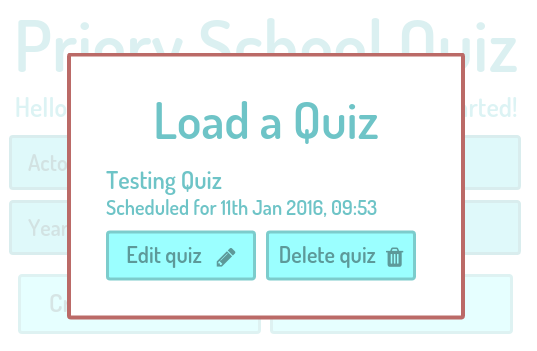
\includegraphics[width=0.95\linewidth]{testing/load_quiz/single_quiz}
  \caption{Single quiz (typical)}
  \label{fig:sub1}
\end{subfigure}%
\begin{subfigure}{0.5\textwidth}
  \centering
  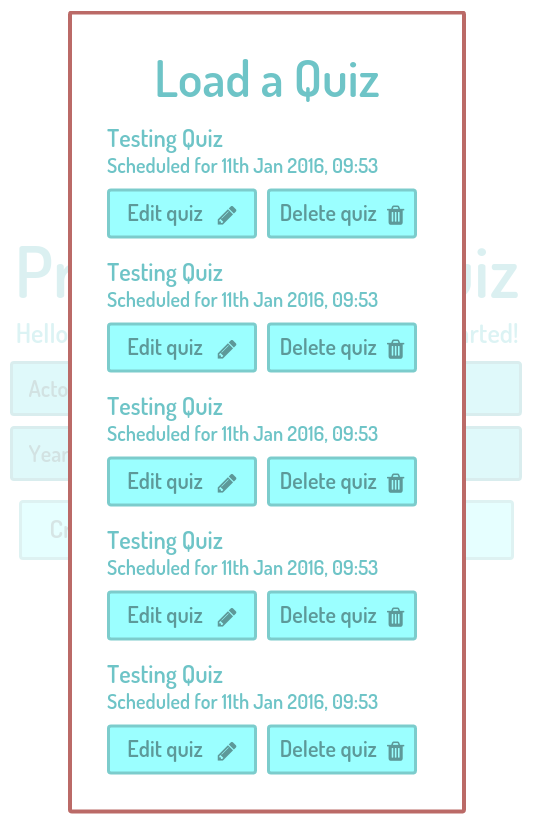
\includegraphics[width=0.95\linewidth]{testing/load_quiz/multiple_quizzes}
  \caption{Five quizzes (extreme)}
  \label{fig:sub2}
\end{subfigure}
\begin{subfigure}{0.5\textwidth}
  \centering
  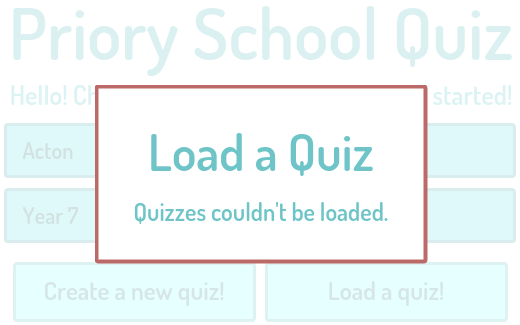
\includegraphics[width=0.95\linewidth]{testing/load_quiz/offline}
  \caption{No connection (erroneous)}
  \label{fig:sub2}
\end{subfigure}
\begin{subfigure}{0.5\textwidth}
  \centering
  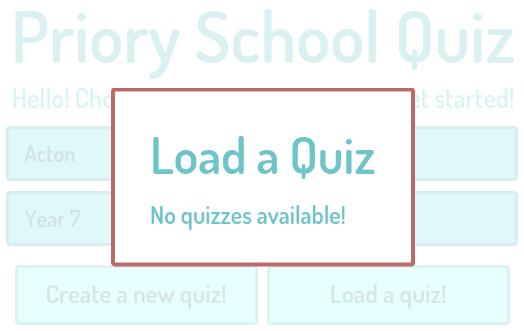
\includegraphics[width=0.95\linewidth]{testing/load_quiz/no_quizzes}
  \caption{No quizzes (null)}
  \label{fig:sub2}
\end{subfigure}
\caption{The load quiz dialog.}
\label{fig:test}
\end{figure}
As can be seen, all the tests have worked successfully: when there is only a single quiz in the database, only a single quiz is shown; when there are five, all of these are listed; when there is no connection, and the system is unable to perform an API call, the correct error message is shown; and when there are simply no quizzes available, this too is properly relayed to the user. \textit{Success.}

\subsection{Create Quiz Test Runs} % (fold)
\label{sub:create_quiz_test}
This section contains the test runs performed on the quiz creator.


\subsubsection{Add Question} % (fold)
\label{ssub:add_question}
This ensures that the user is able to succesfully add a new question to the current quiz when the add question button is pressed.
\begin{figure}[!htbp]
\centering
\begin{subfigure}{0.5\textwidth}
  \centering
  \includegraphics[width=0.95\linewidth]{testing/create_quiz/add_question/before}
  \caption{Before}
  \label{fig:sub1}
\end{subfigure}%
\begin{subfigure}{0.5\textwidth}
  \centering
  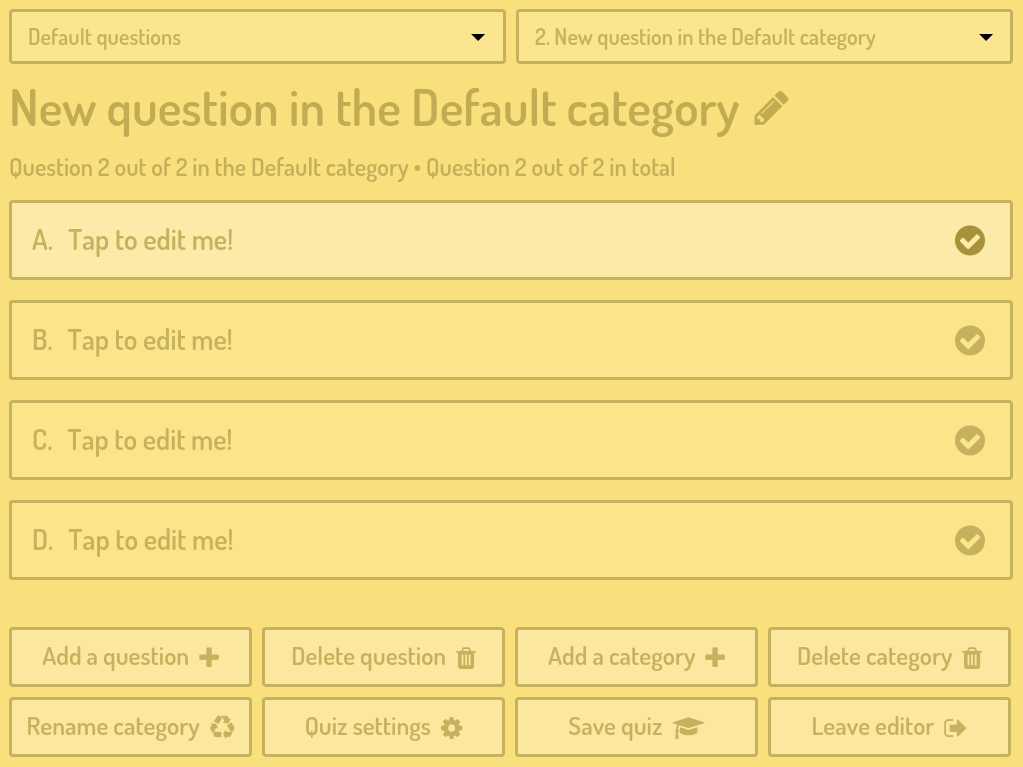
\includegraphics[width=0.95\linewidth]{testing/create_quiz/add_question/after}
  \caption{After}
  \label{fig:sub2}
\end{subfigure}
\caption{Adding a question to the quiz.}
\label{fig:test}
\end{figure}
\\As the two pictures indicate, after pressing the add question button, a new question was added to the system, and this was reflectd in the label unde the question title. \textit{Success.}
% subsubsection add_question (end)

\clearpage

\subsubsection{Edit Question} % (fold)
\label{ssub:edit_question}
This ensures that the user is able to succesfully edit a question in the current quiz.
\begin{figure}[!htbp]
\begin{subfigure}{0.5\textwidth}
  \centering
  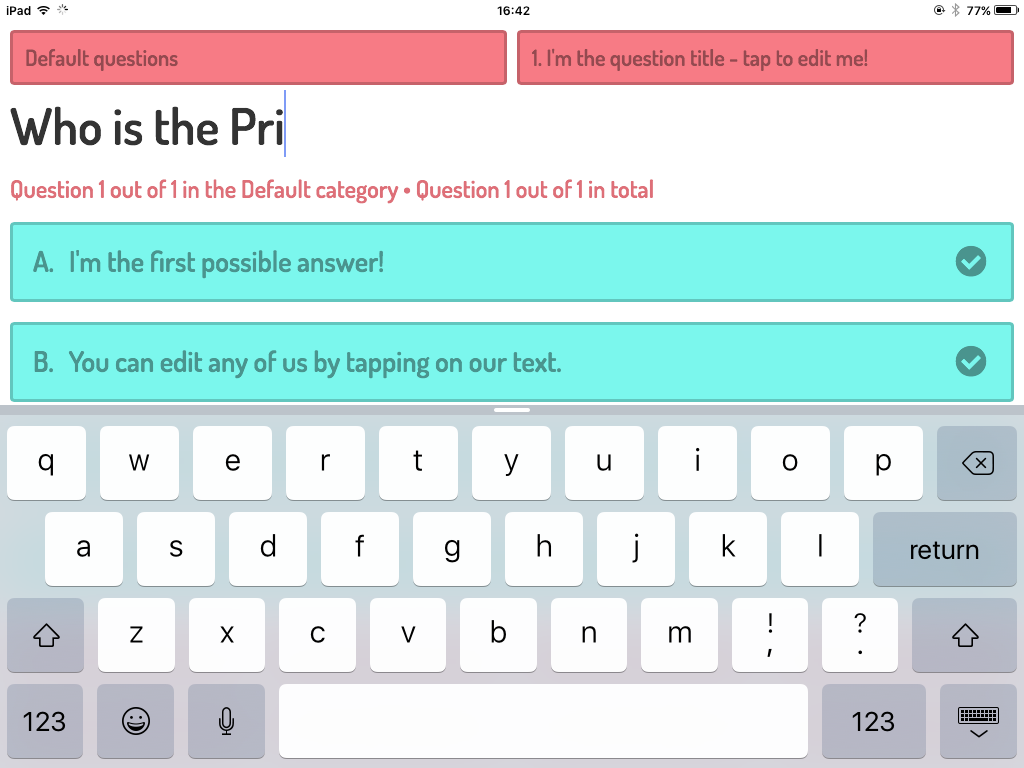
\includegraphics[width=0.95\linewidth]{testing/create_quiz/edit_question/during}
  \caption{During}
  \label{fig:sub2}
\end{subfigure}
\begin{subfigure}{0.5\textwidth}
  \centering
  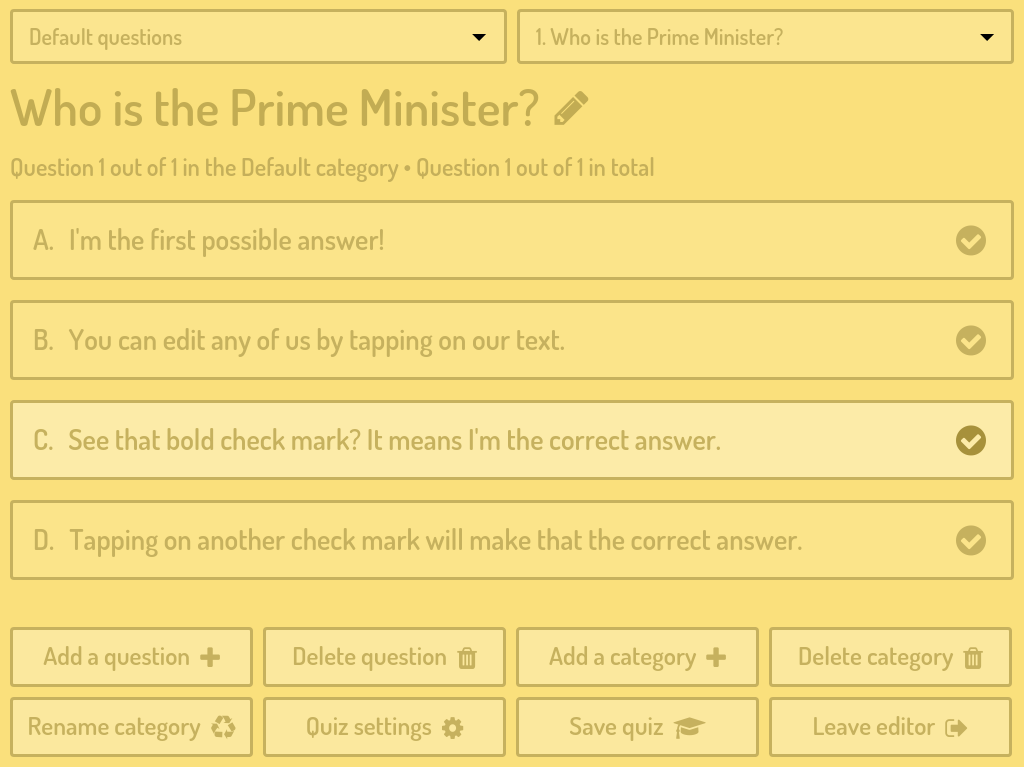
\includegraphics[width=0.95\linewidth]{testing/create_quiz/edit_question/after}
  \caption{After}
  \label{fig:sub3}
\end{subfigure}
\caption{Editing a question to the quiz.}
\label{fig:test}
\end{figure}
% subsubsection edit_question (end)


\subsubsection{Delete Question} % (fold)
\label{ssub:delete_question}
This ensures that the user is able to succesfully delete their questions from the current quiz.
\\\\\textit{\textbf{Note:} In order to prove that the question has actually been deleted, the screenshot captures the developer tools used in the creation of the application; an action showing that the question has been deleted is clearly visible.}
\begin{figure}[!htbp]
\centering
\begin{subfigure}{0.5\textwidth}
  \centering
  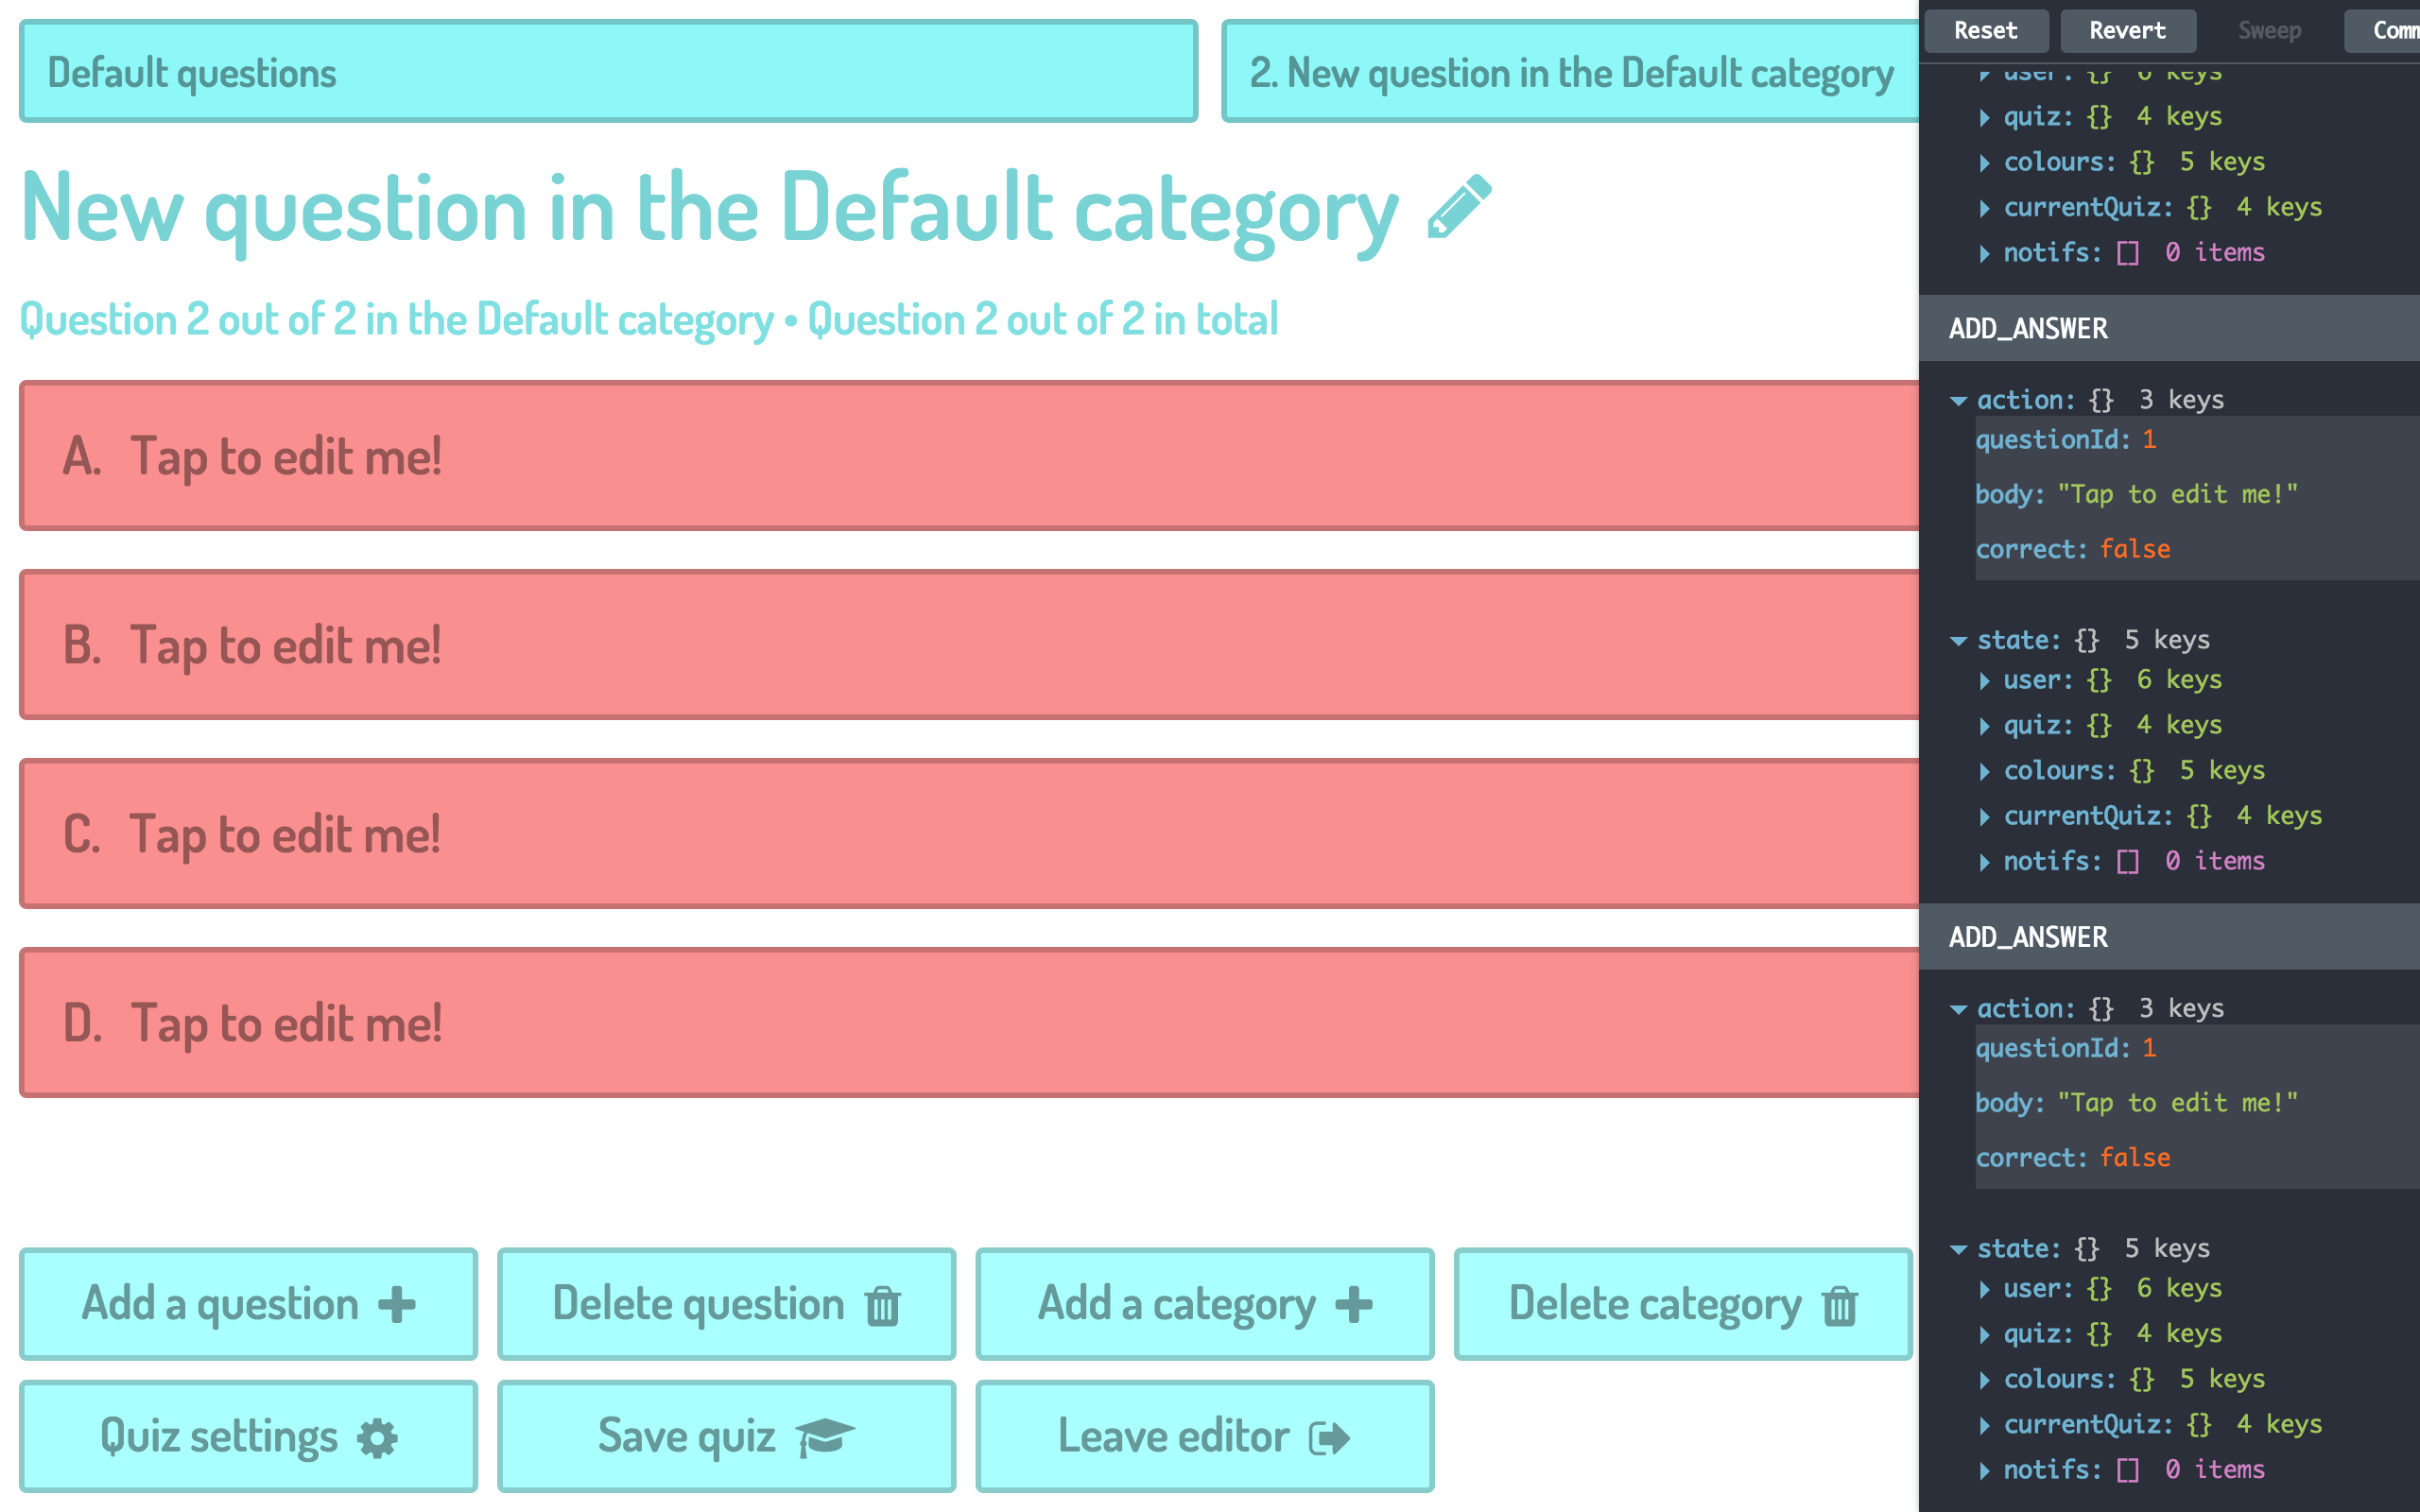
\includegraphics[width=0.95\linewidth]{testing/create_quiz/delete_question/before}
  \caption{Before}
  \label{fig:sub1}
\end{subfigure}%
\begin{subfigure}{0.5\textwidth}
  \centering
  \includegraphics[width=0.95\linewidth]{testing/create_quiz/delete_question/after}
  \caption{After}
  \label{fig:sub2}
\end{subfigure}
\caption{Delete a question in the quiz.}
\label{fig:test}
\end{figure}
\\The second screenshot shows that a delete question action was passed to the quiz reducer, resulting in the question being successfully deleted; this is also reflected in the labels. \textit{Success.}
% subsubsection delete_question (end)


\subsubsection{Add Category} % (fold)
\label{ssub:add_category}
This ensures that the user is able to succesfully add a custom category to the current quiz.
\begin{figure}[!htbp]
\centering
\begin{subfigure}{0.5\textwidth}
  \centering
  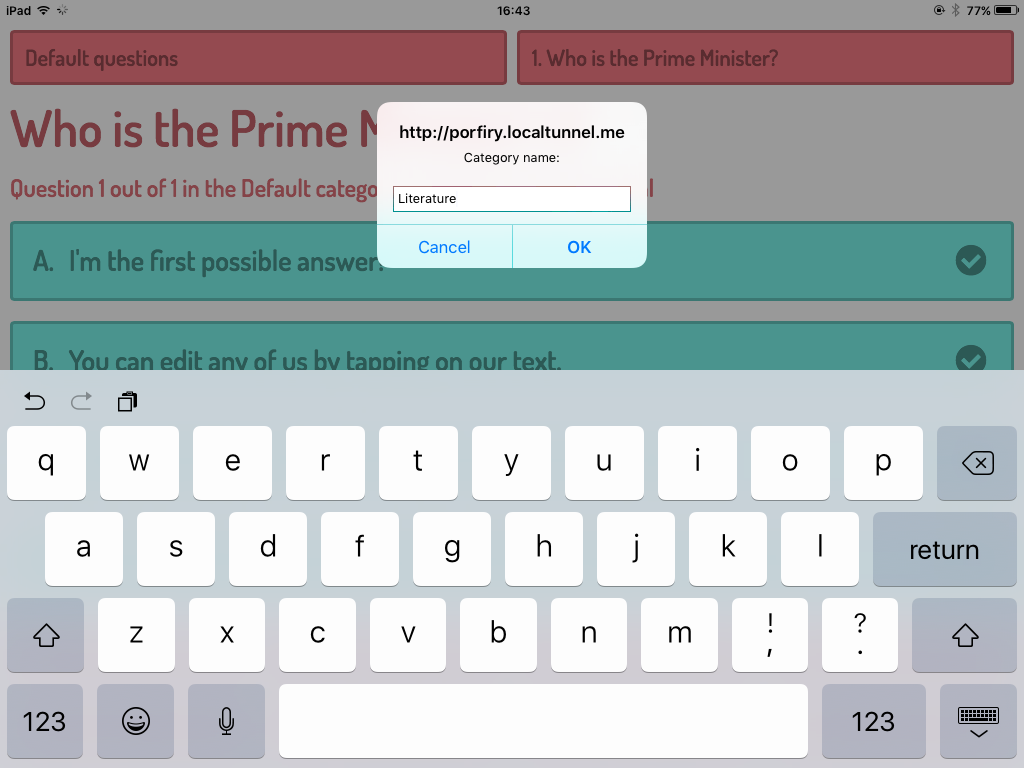
\includegraphics[width=0.95\linewidth]{testing/create_quiz/add_category/during}
  \caption{During}
  \label{fig:sub1}
\end{subfigure}%
\begin{subfigure}{0.5\textwidth}
  \centering
  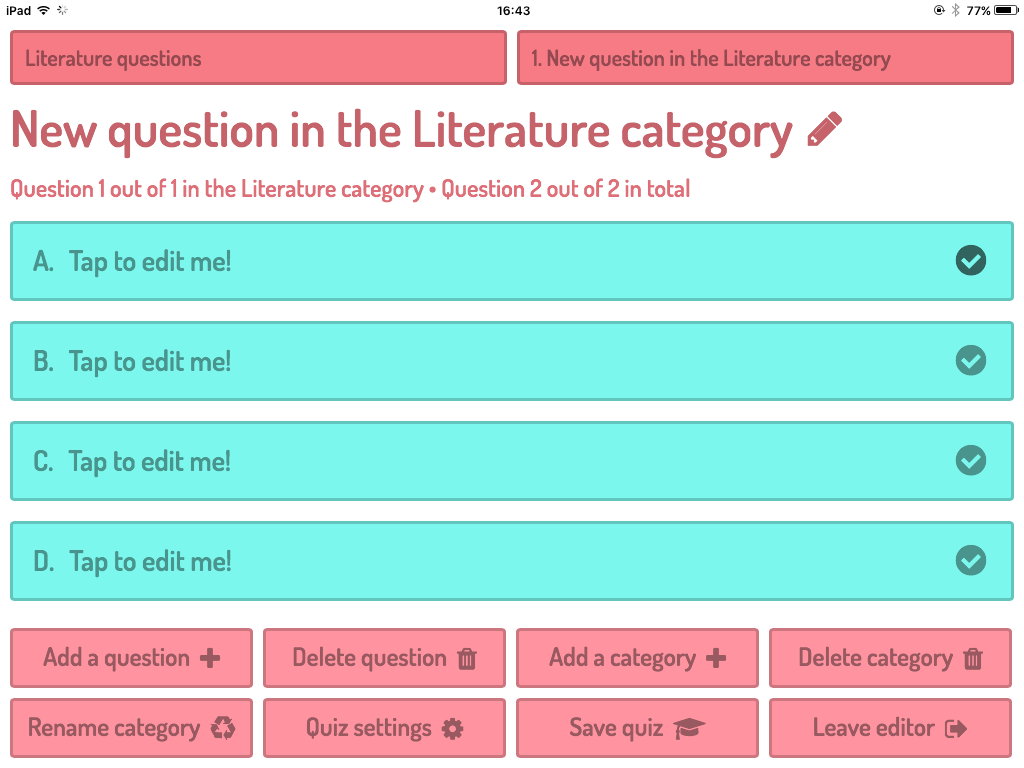
\includegraphics[width=0.95\linewidth]{testing/create_quiz/add_category/after}
  \caption{After}
  \label{fig:sub2}
\end{subfigure}
\caption{Adding a category to the quiz.}
\label{fig:test}
\end{figure}
As expected, a dialog to enter a category name is shown when the add category button is pressed, and the new category is added successfully. \textit{Success.}
% subsubsection add_category (end)


\subsubsection{Delete Category} % (fold)
\label{ssub:add_category}
This ensures that the user is able to succesfully delete their custom categories in the current quiz.
\begin{figure}[!htbp]
\centering
\begin{subfigure}{0.5\textwidth}
  \centering
  \includegraphics[width=0.95\linewidth]{testing/create_quiz/delete_category/before}
  \caption{Before}
  \label{fig:sub1}
\end{subfigure}%
\begin{subfigure}{0.5\textwidth}
  \centering
  \includegraphics[width=0.95\linewidth]{testing/create_quiz/delete_category/after}
  \caption{After}
  \label{fig:sub2}
\end{subfigure}
\caption{Deleting a category from the quiz.}
\label{fig:test}
\end{figure}
As expected, a dialog to enter a category name is shown when the add category button is pressed, and the new category is added successfully. \textit{Success.}
% subsubsection add_category (end)


\subsubsection{Rename Category} % (fold)
\label{ssub:add_category}
This ensures that the user is able to succesfully rename their custom categories in the current quiz.
\begin{figure}[!htbp]
\centering
\begin{subfigure}{0.5\textwidth}
  \centering
  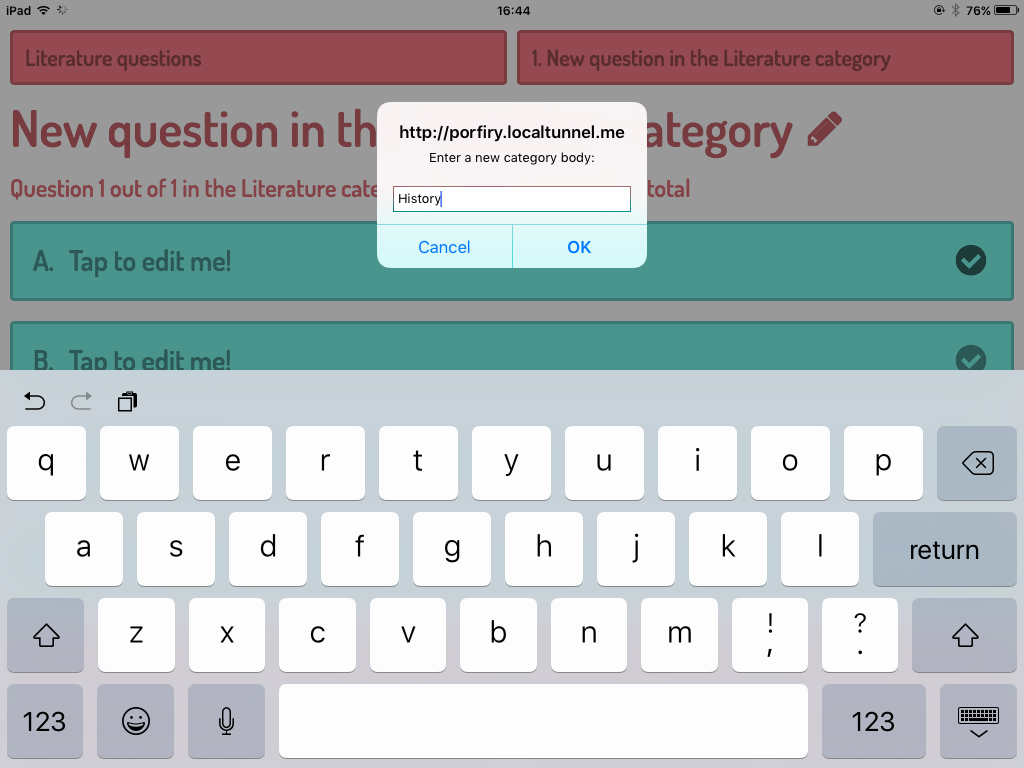
\includegraphics[width=0.95\linewidth]{testing/create_quiz/rename_category/during}
  \caption{During}
  \label{fig:sub1}
\end{subfigure}%
\begin{subfigure}{0.5\textwidth}
  \centering
  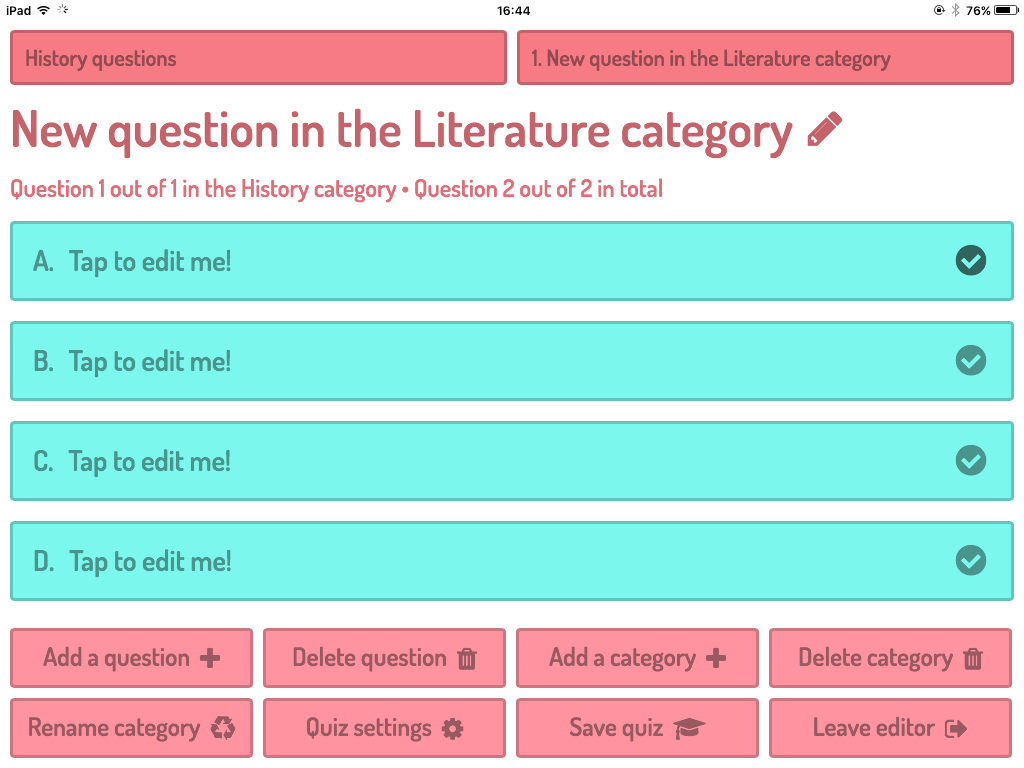
\includegraphics[width=0.95\linewidth]{testing/create_quiz/rename_category/after}
  \caption{After}
  \label{fig:sub2}
\end{subfigure}
\caption{Renaming a category in the quiz.}
\label{fig:test}
\end{figure}
As expected, a dialog to enter the new category name is shown when the rename category button is pressed, and category is renamed successfully. \textit{Success.}
% subsubsection add_category (end)

\subsubsection{Edit Answer} % (fold)
\label{ssub:add_category}
This test ensures that the user is able to edit the body of an answer in the current quiz.
\begin{figure}[!htbp]
\centering
\begin{subfigure}{0.5\textwidth}
  \centering
  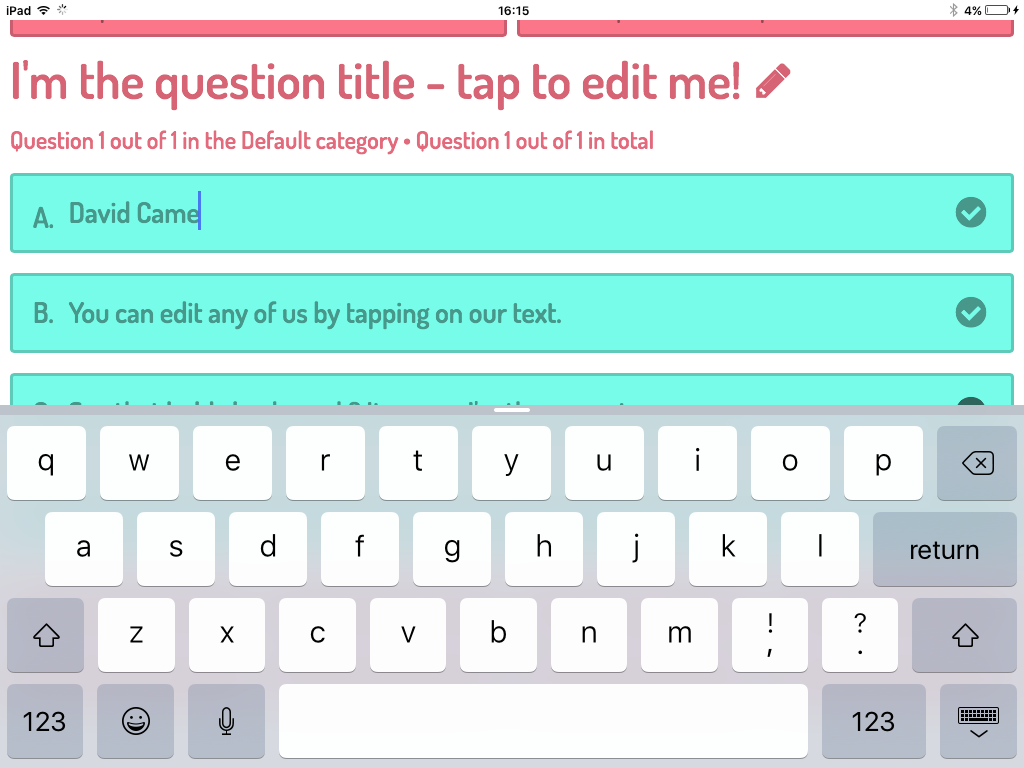
\includegraphics[width=0.95\linewidth]{testing/create_quiz/edit_answer/during}
  \caption{During}
  \label{fig:sub1}
\end{subfigure}%
\begin{subfigure}{0.5\textwidth}
  \centering
  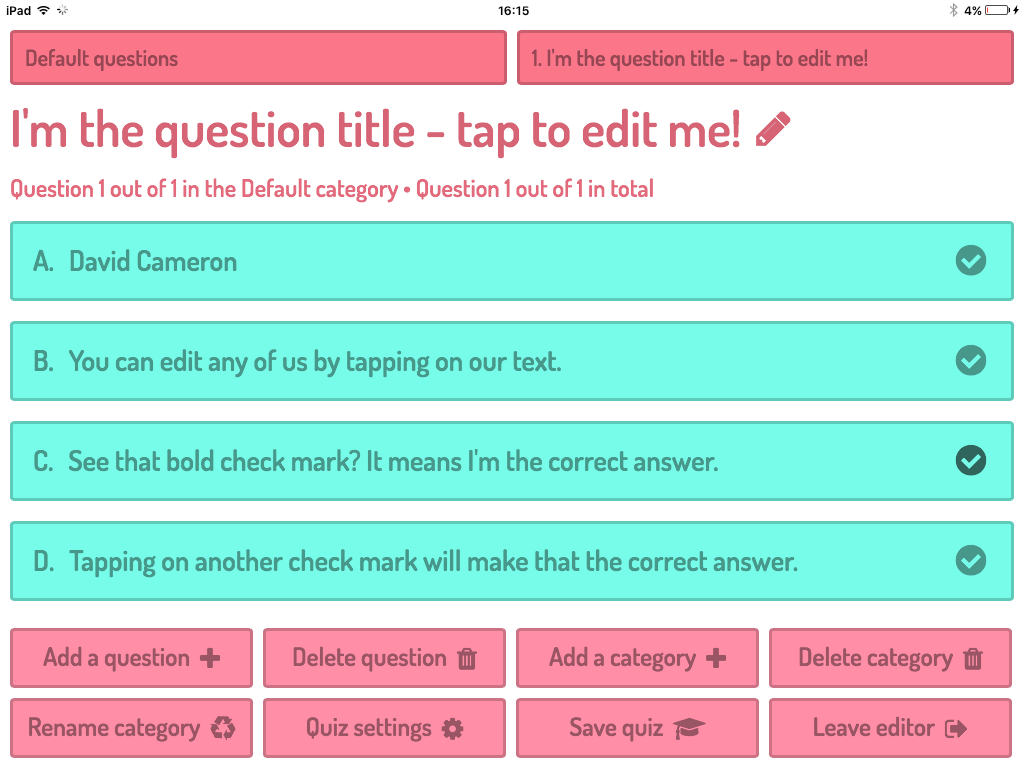
\includegraphics[width=0.95\linewidth]{testing/create_quiz/edit_answer/after}
  \caption{After}
  \label{fig:sub2}
\end{subfigure}
\caption{Marking an answer in as correct.}
\label{fig:test}
\end{figure}
\\As expected, the application allowed for the answer body to be edited, and then persisted this change after leaving the edit mode. \textit{Success.}
% subsubsection add_category (end)


\subsubsection{Mark Answer as Correct} % (fold)
\label{ssub:add_category}
This ensures that the user is able to succesfully mark an answer as correct in the current quiz.
\begin{figure}[!htbp]
\centering
\begin{subfigure}{0.5\textwidth}
  \centering
  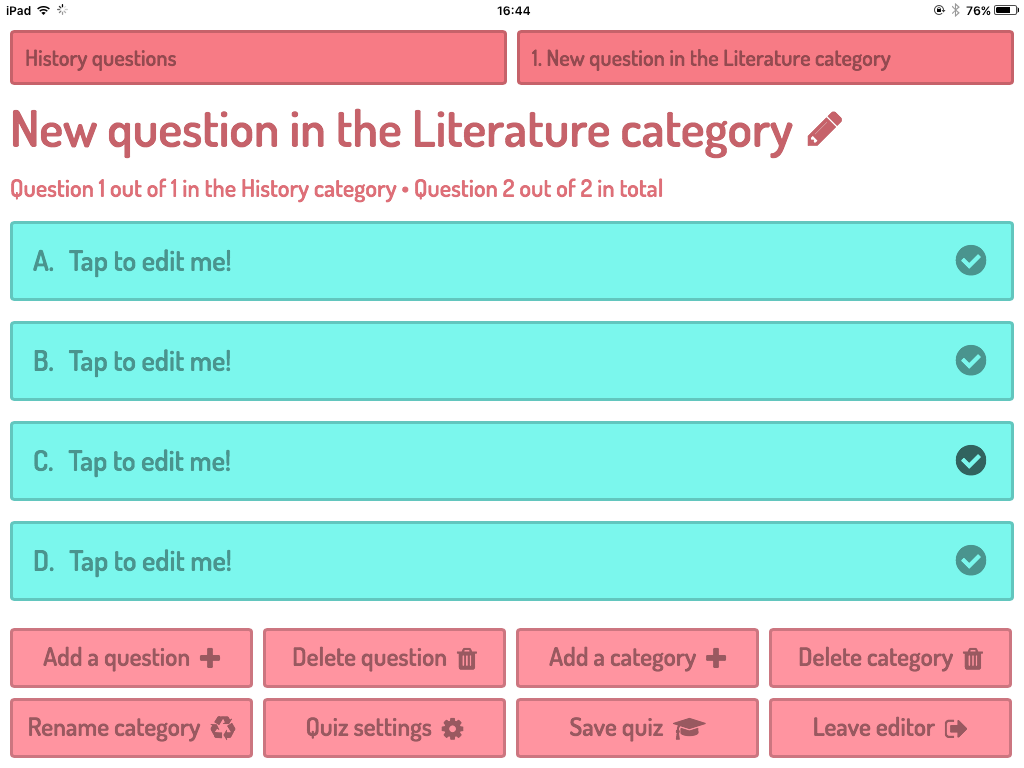
\includegraphics[width=0.95\linewidth]{testing/create_quiz/change_answer/before}
  \caption{During}
  \label{fig:sub1}
\end{subfigure}%
\begin{subfigure}{0.5\textwidth}
  \centering
  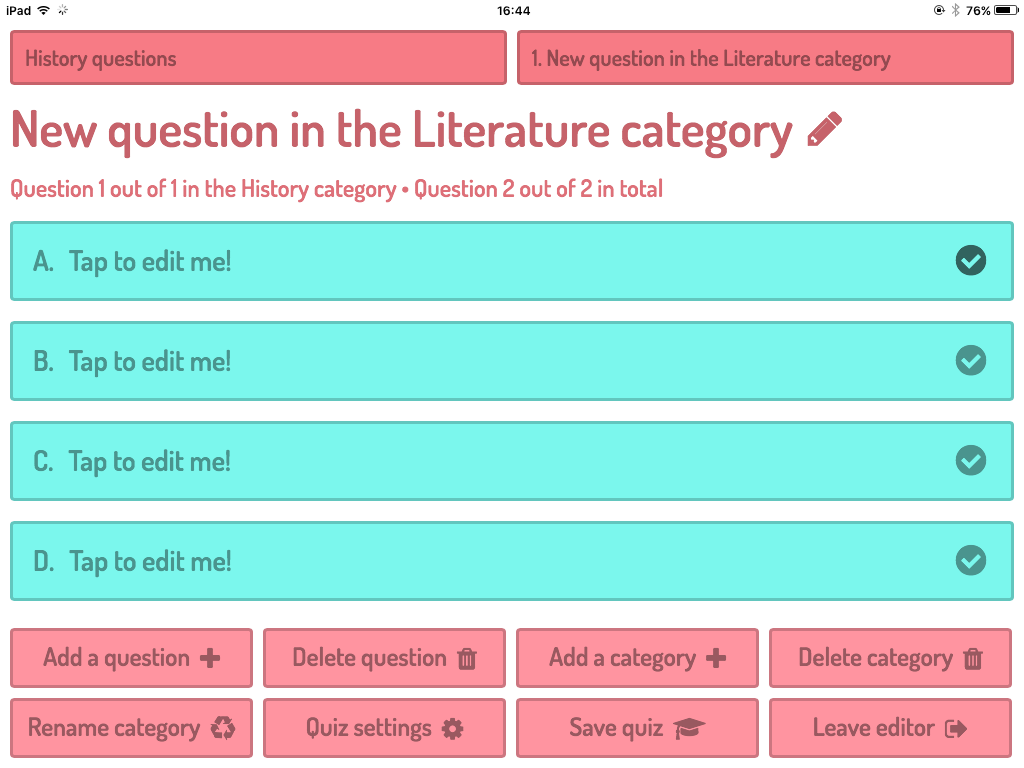
\includegraphics[width=0.95\linewidth]{testing/create_quiz/change_answer/after}
  \caption{After}
  \label{fig:sub2}
\end{subfigure}
\caption{Marking an answer in as correct.}
\label{fig:test}
\end{figure}
\\As expected, the correct mark moved from the third to the first question, meaning that it was marked as correct. \textit{Success.}
% subsubsection add_category (end)


\subsubsection{Save Quiz} % (fold)
\label{ssub:add_category}
This test ensures that the user is able to save their quizzes to the database.
\begin{figure}[!htbp]
\centering
\begin{subfigure}{0.5\textwidth}
  \centering
  \includegraphics[width=0.95\linewidth]{testing/create_quiz/save_quiz/before}
  \caption{During}
  \label{fig:sub1}
\end{subfigure}%
\begin{subfigure}{0.5\textwidth}
  \centering
  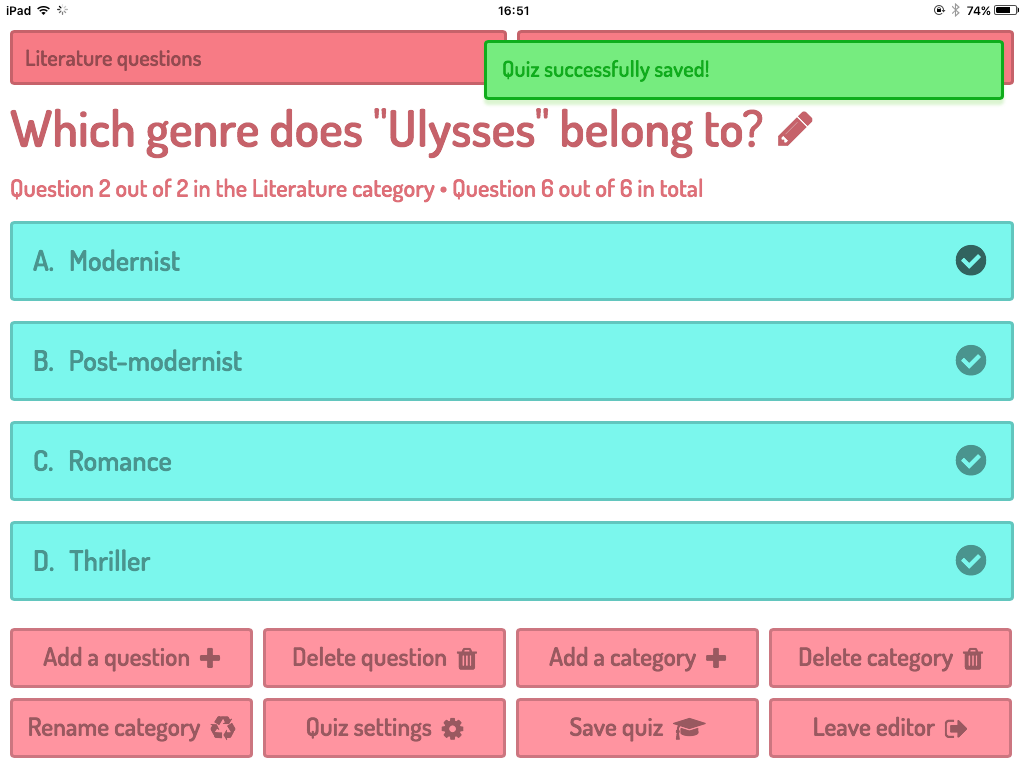
\includegraphics[width=0.95\linewidth]{testing/create_quiz/save_quiz/after}
  \caption{After}
  \label{fig:sub2}
\end{subfigure}
\caption{Saving a quiz to the database.}
\label{fig:test}
\end{figure}
\\As expected, the correct mark moved from the third to the first question, meaning that it was marked as correct. \textit{Success.}
% subsubsection add_category (end)

\subsubsection{Move Questions on Time}
This test ensures that the quiz moves to the correct questions at the correct time, using the test quiz specified in the test plan. Due to the difficulty of taking valid screenshots of this process, a table is included below with room for a teacher to sign as confirmation that this functionality is working.

\begin{table}[]
\centering
\begin{tabular}{|l|l|l|}
\hline
\multicolumn{1}{|c|}{\textbf{Expected result}}              & \multicolumn{1}{c|}{\textbf{Works}} & \multicolumn{1}{c|}{\textbf{Signature}} \\ \hline
Displays "Who is the French Premier?" at 0-10 seconds       & Yes                                 &                                         \\ \hline
Displays "Who won the 1960 World Cup?" at 10-20 seconds     & Yes                                 &                                         \\ \hline
Displays "What is the capital of Iceland?" at 20-30 seconds & Yes                                 &                                         \\ \hline
\end{tabular}
\caption{My caption}
\label{my-label}
\end{table}

\\As can be witnessed, the quiz moves to the correct questions at the correct time, meaning that the test has passed. \texit{Success.}

\subsection{Results Test Runs} % (fold)
\label{sub:results_test_runs}
This section tests that the results screen works correctly.

\subsubsection{Connects to State Store} % (fold)
\label{ssub:connects_to_state_store}
This test ensures that the component can connect to the state store.
% subsubsection connects_to_state_store (end)

\subsubsection{Display Correct Results} % (fold)
\label{ssub:display_correct_results}
This test ensures that the results screen shows the correct results.
% subsubsection display_correct_results (end)
% subsection results_test_runs (end)


% Import test_runs
\clearpage
\section{Test Runs}
These are the actual test runs, indicating whether or not a test has successfully completed. For each test, the unit test code is included, followed by a screenshot of the test outcome. If a test is unsuccessful, the changes made to the code will be shown, followed by another screenshot of the test outcome.

\subsection{Login Test Runs}
This subsection contains the test runs for the login screen, using as a reference the login screen test plan available at 13.1.

\subsubsection{Load Quizzes}
This test ensures that a list of all available quizzes can be searched for and found on the login screen, ready to either edit or delete.

\begin{figure}[!htbp]
\centering
\begin{subfigure}{0.5\textwidth}
  \centering
  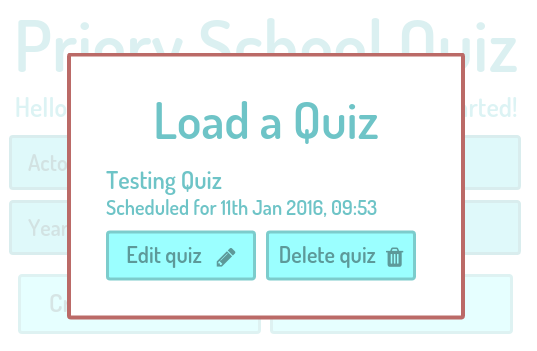
\includegraphics[width=0.95\linewidth]{testing/load_quiz/single_quiz}
  \caption{Single quiz (typical)}
  \label{fig:sub1}
\end{subfigure}%
\begin{subfigure}{0.5\textwidth}
  \centering
  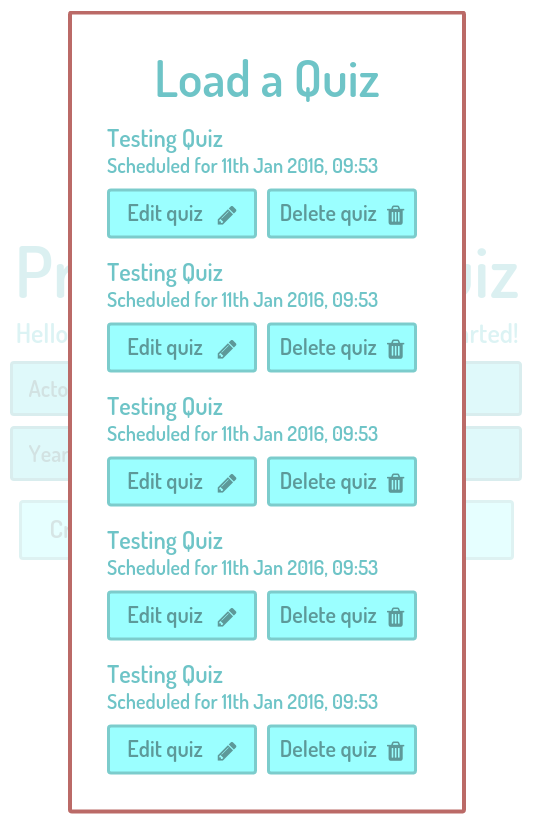
\includegraphics[width=0.95\linewidth]{testing/load_quiz/multiple_quizzes}
  \caption{Five quizzes (extreme)}
  \label{fig:sub2}
\end{subfigure}
\begin{subfigure}{0.5\textwidth}
  \centering
  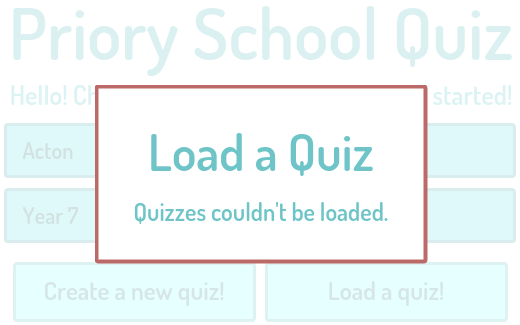
\includegraphics[width=0.95\linewidth]{testing/load_quiz/offline}
  \caption{No connection (erroneous)}
  \label{fig:sub2}
\end{subfigure}
\begin{subfigure}{0.5\textwidth}
  \centering
  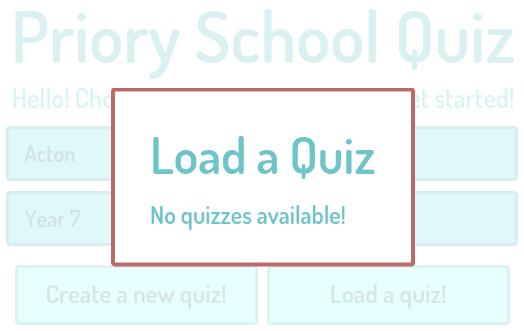
\includegraphics[width=0.95\linewidth]{testing/load_quiz/no_quizzes}
  \caption{No quizzes (null)}
  \label{fig:sub2}
\end{subfigure}
\caption{The load quiz dialog.}
\label{fig:test}
\end{figure}
As can be seen, all the tests have worked successfully: when there is only a single quiz in the database, only a single quiz is shown; when there are five, all of these are listed; when there is no connection, and the system is unable to perform an API call, the correct error message is shown; and when there are simply no quizzes available, this too is properly relayed to the user. \textit{Success.}

\subsection{Create Quiz Test Runs} % (fold)
\label{sub:create_quiz_test}
This section contains the test runs performed on the quiz creator.


\subsubsection{Add Question} % (fold)
\label{ssub:add_question}
This ensures that the user is able to succesfully add a new question to the current quiz when the add question button is pressed.
\begin{figure}[!htbp]
\centering
\begin{subfigure}{0.5\textwidth}
  \centering
  \includegraphics[width=0.95\linewidth]{testing/create_quiz/add_question/before}
  \caption{Before}
  \label{fig:sub1}
\end{subfigure}%
\begin{subfigure}{0.5\textwidth}
  \centering
  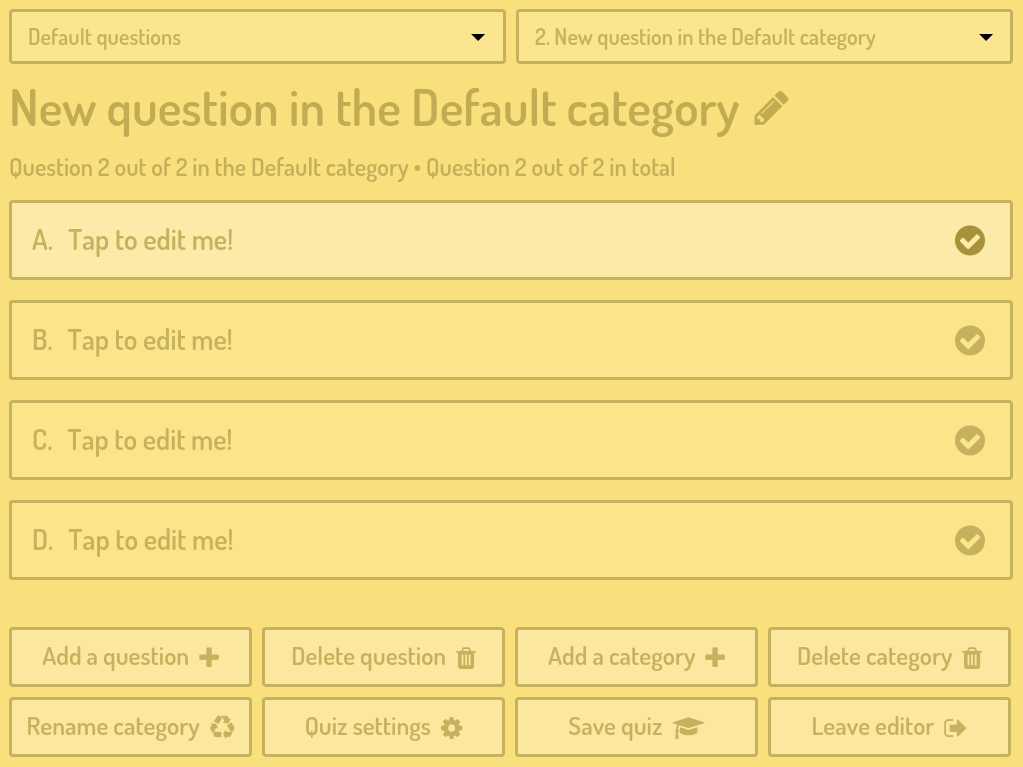
\includegraphics[width=0.95\linewidth]{testing/create_quiz/add_question/after}
  \caption{After}
  \label{fig:sub2}
\end{subfigure}
\caption{Adding a question to the quiz.}
\label{fig:test}
\end{figure}
\\As the two pictures indicate, after pressing the add question button, a new question was added to the system, and this was reflectd in the label unde the question title. \textit{Success.}
% subsubsection add_question (end)

\clearpage

\subsubsection{Edit Question} % (fold)
\label{ssub:edit_question}
This ensures that the user is able to succesfully edit a question in the current quiz.
\begin{figure}[!htbp]
\begin{subfigure}{0.5\textwidth}
  \centering
  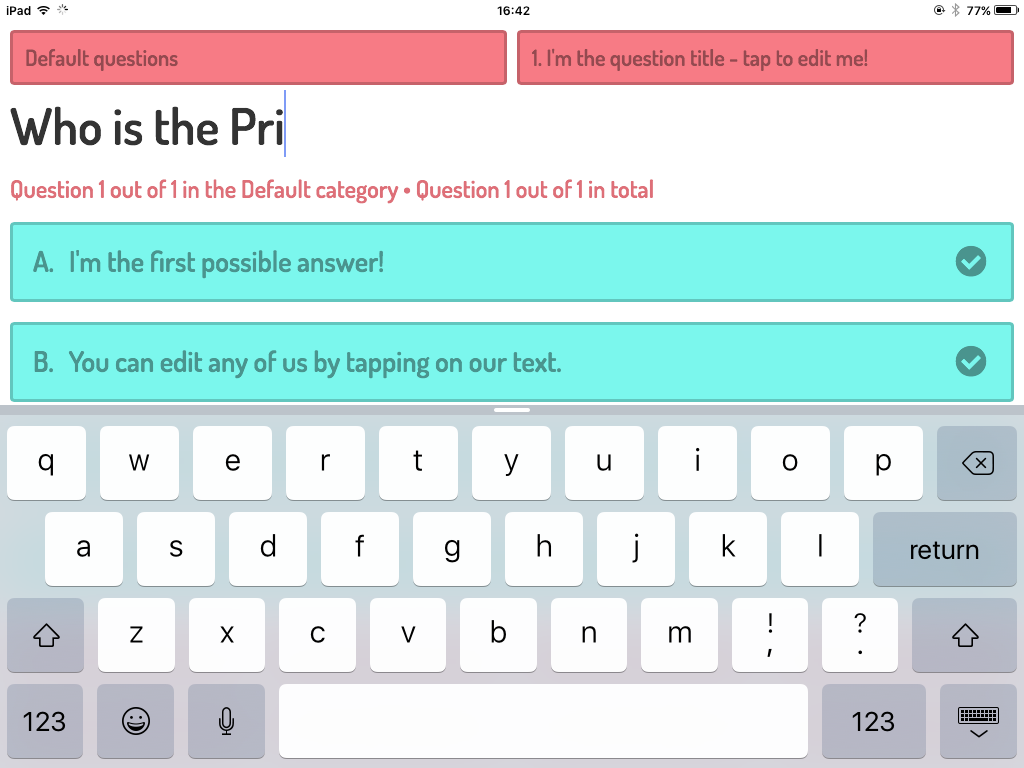
\includegraphics[width=0.95\linewidth]{testing/create_quiz/edit_question/during}
  \caption{During}
  \label{fig:sub2}
\end{subfigure}
\begin{subfigure}{0.5\textwidth}
  \centering
  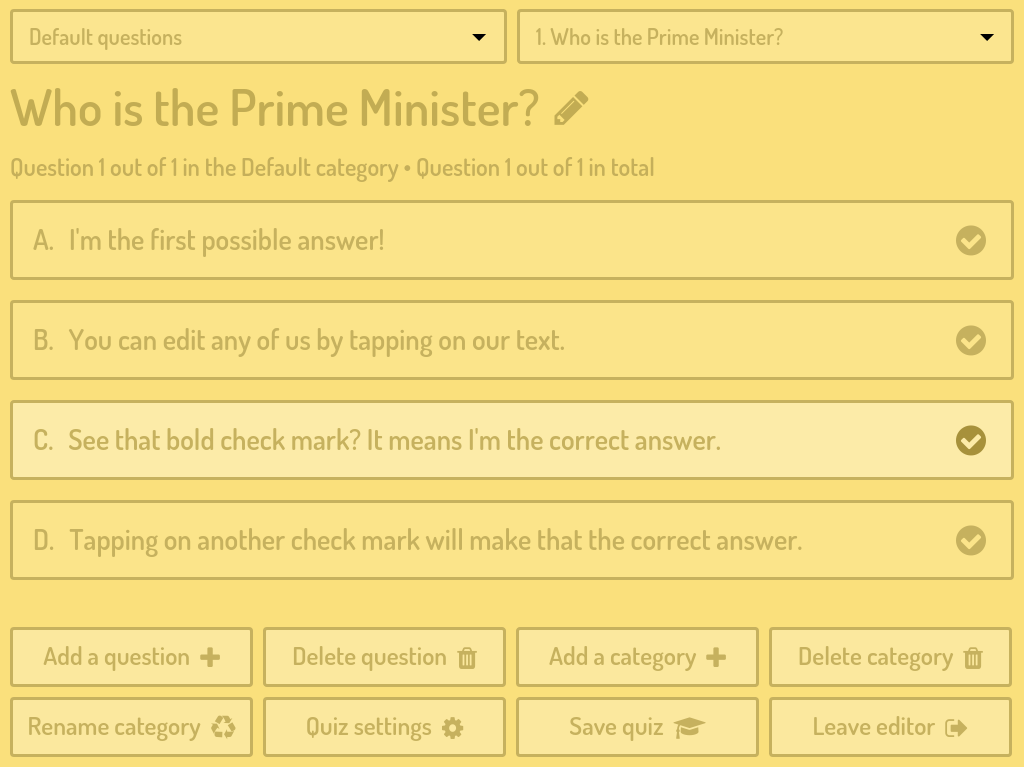
\includegraphics[width=0.95\linewidth]{testing/create_quiz/edit_question/after}
  \caption{After}
  \label{fig:sub3}
\end{subfigure}
\caption{Editing a question to the quiz.}
\label{fig:test}
\end{figure}
% subsubsection edit_question (end)


\subsubsection{Delete Question} % (fold)
\label{ssub:delete_question}
This ensures that the user is able to succesfully delete their questions from the current quiz.
\\\\\textit{\textbf{Note:} In order to prove that the question has actually been deleted, the screenshot captures the developer tools used in the creation of the application; an action showing that the question has been deleted is clearly visible.}
\begin{figure}[!htbp]
\centering
\begin{subfigure}{0.5\textwidth}
  \centering
  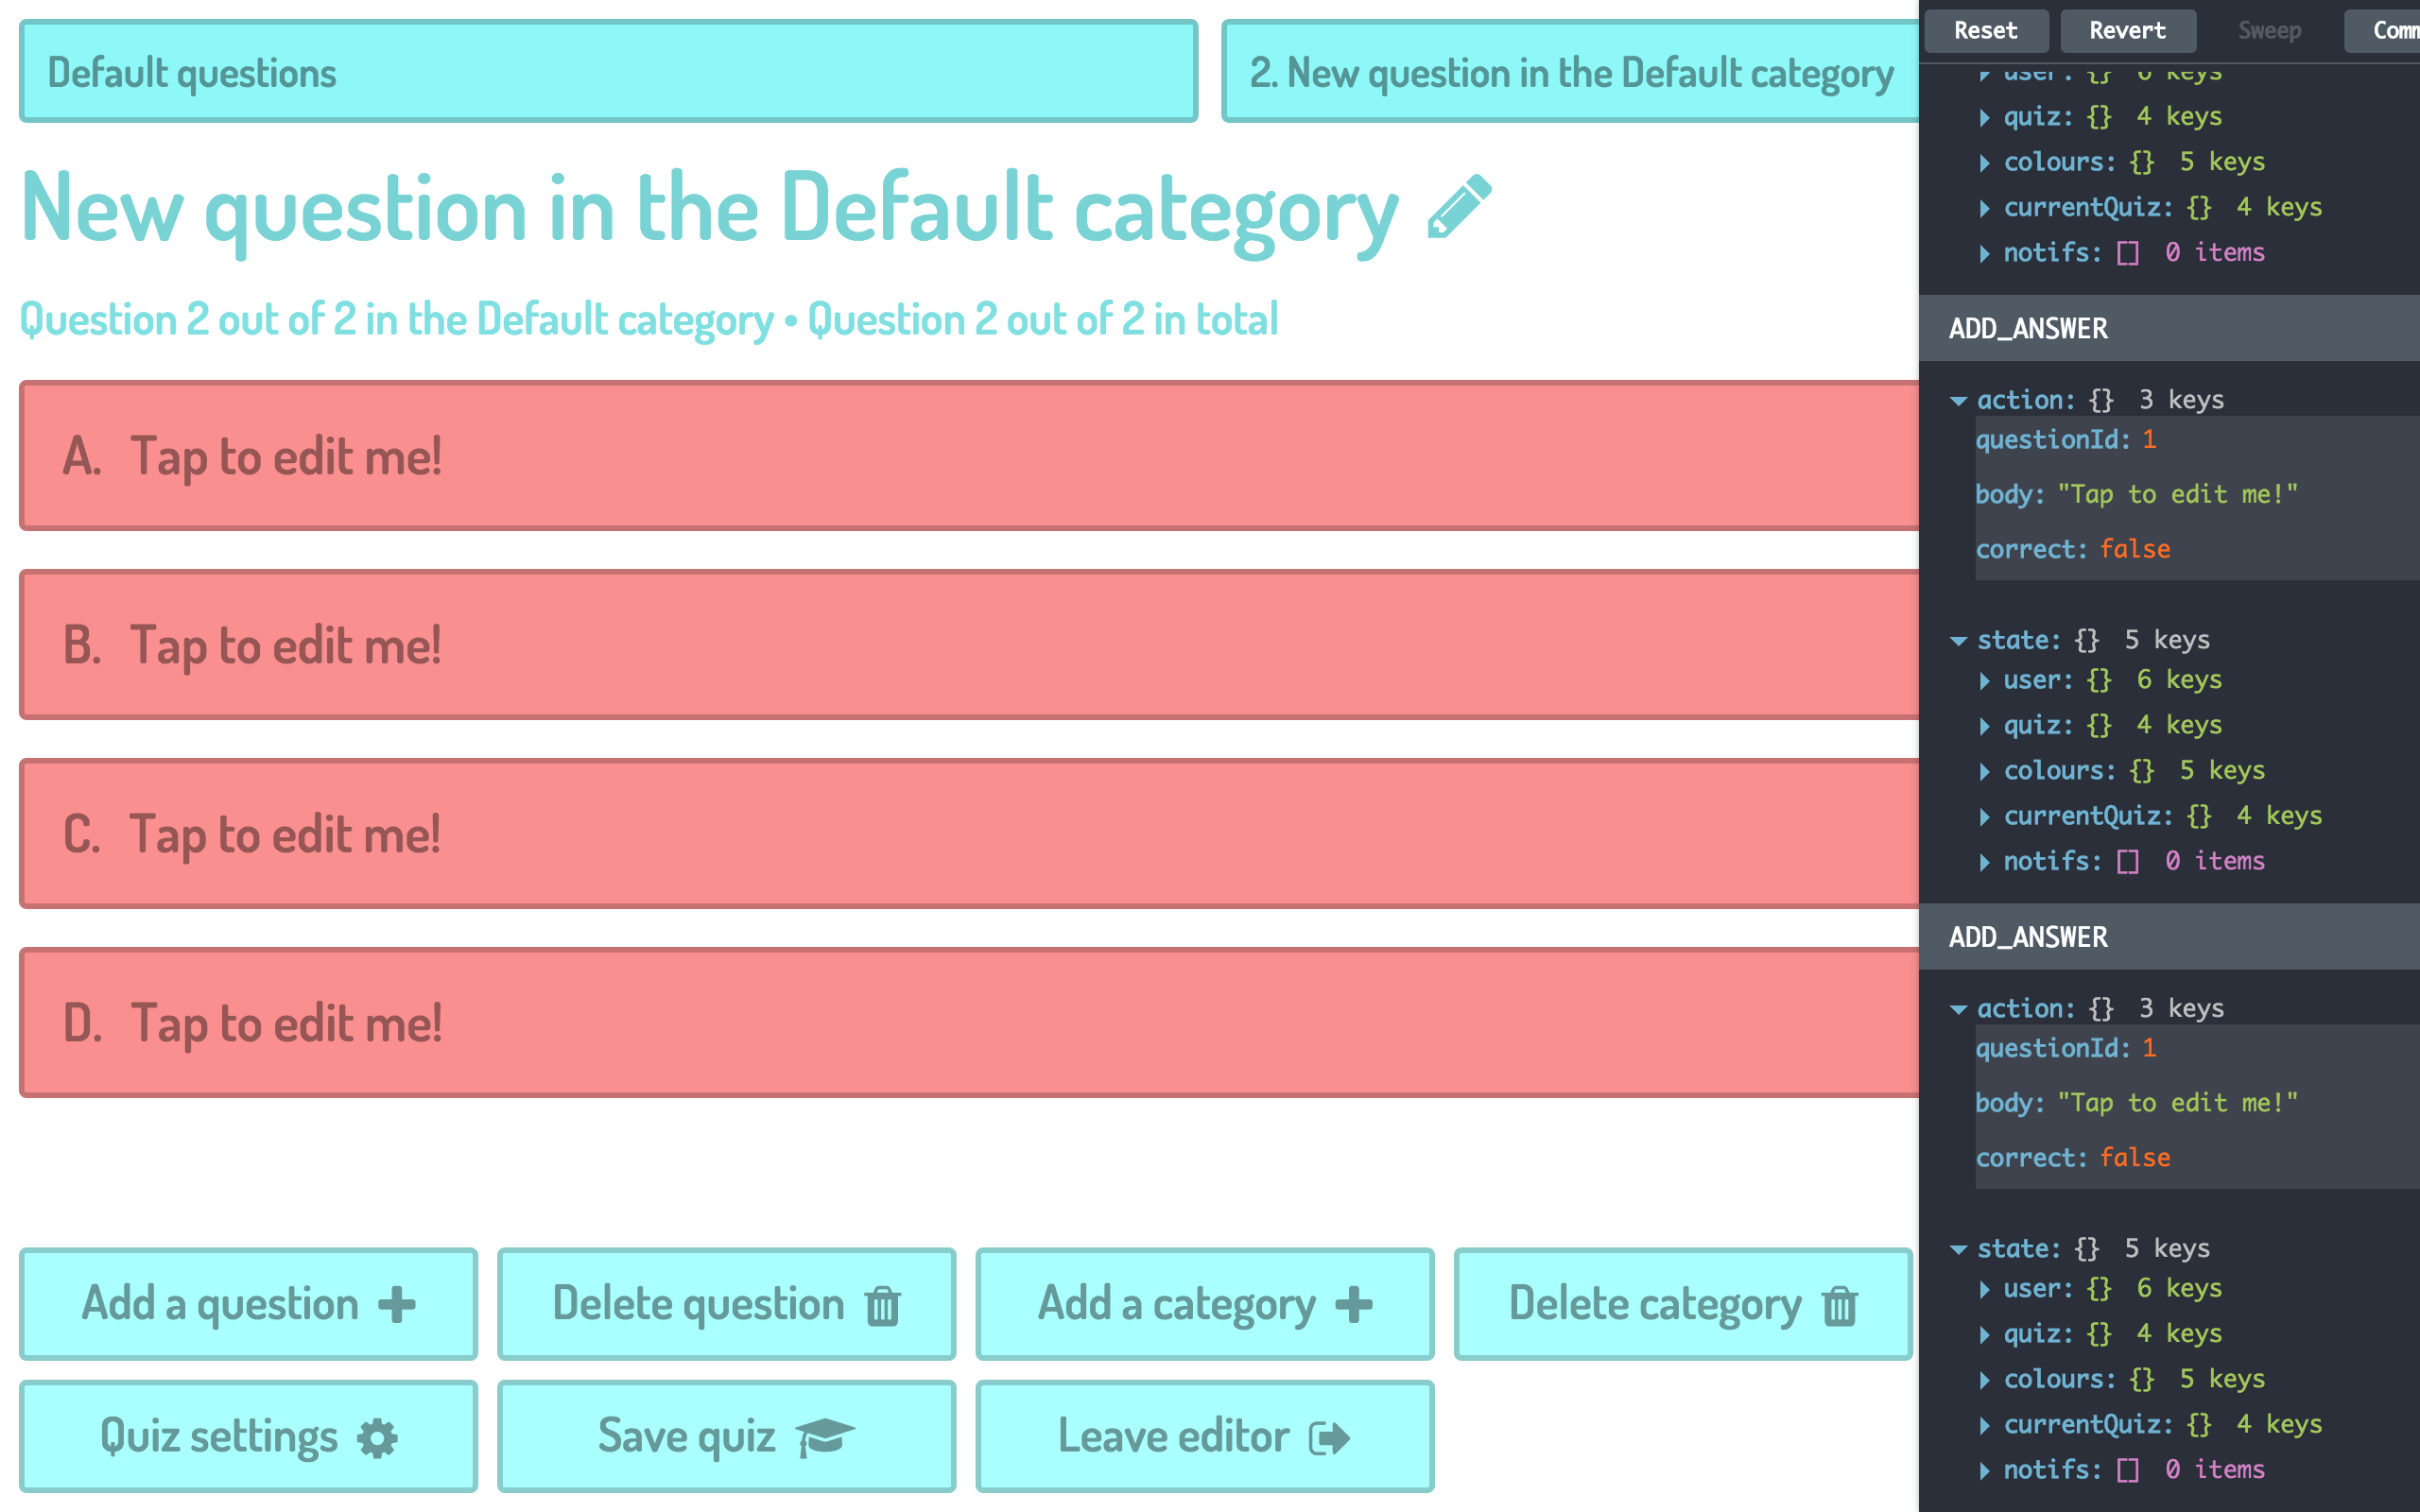
\includegraphics[width=0.95\linewidth]{testing/create_quiz/delete_question/before}
  \caption{Before}
  \label{fig:sub1}
\end{subfigure}%
\begin{subfigure}{0.5\textwidth}
  \centering
  \includegraphics[width=0.95\linewidth]{testing/create_quiz/delete_question/after}
  \caption{After}
  \label{fig:sub2}
\end{subfigure}
\caption{Delete a question in the quiz.}
\label{fig:test}
\end{figure}
\\The second screenshot shows that a delete question action was passed to the quiz reducer, resulting in the question being successfully deleted; this is also reflected in the labels. \textit{Success.}
% subsubsection delete_question (end)


\subsubsection{Add Category} % (fold)
\label{ssub:add_category}
This ensures that the user is able to succesfully add a custom category to the current quiz.
\begin{figure}[!htbp]
\centering
\begin{subfigure}{0.5\textwidth}
  \centering
  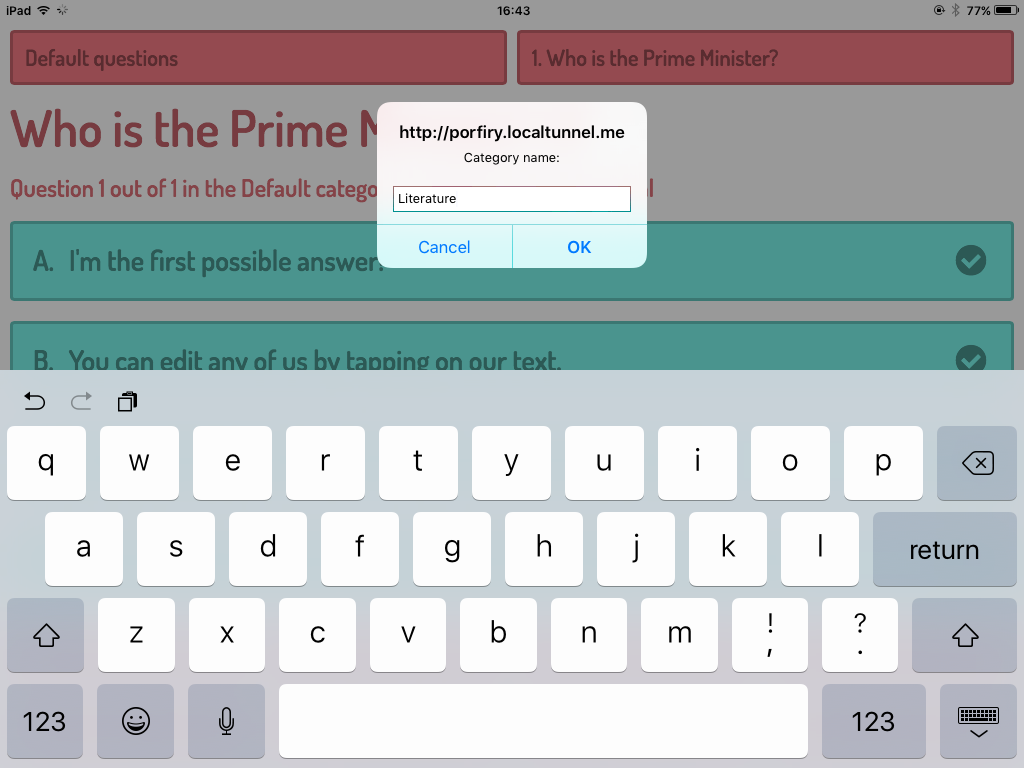
\includegraphics[width=0.95\linewidth]{testing/create_quiz/add_category/during}
  \caption{During}
  \label{fig:sub1}
\end{subfigure}%
\begin{subfigure}{0.5\textwidth}
  \centering
  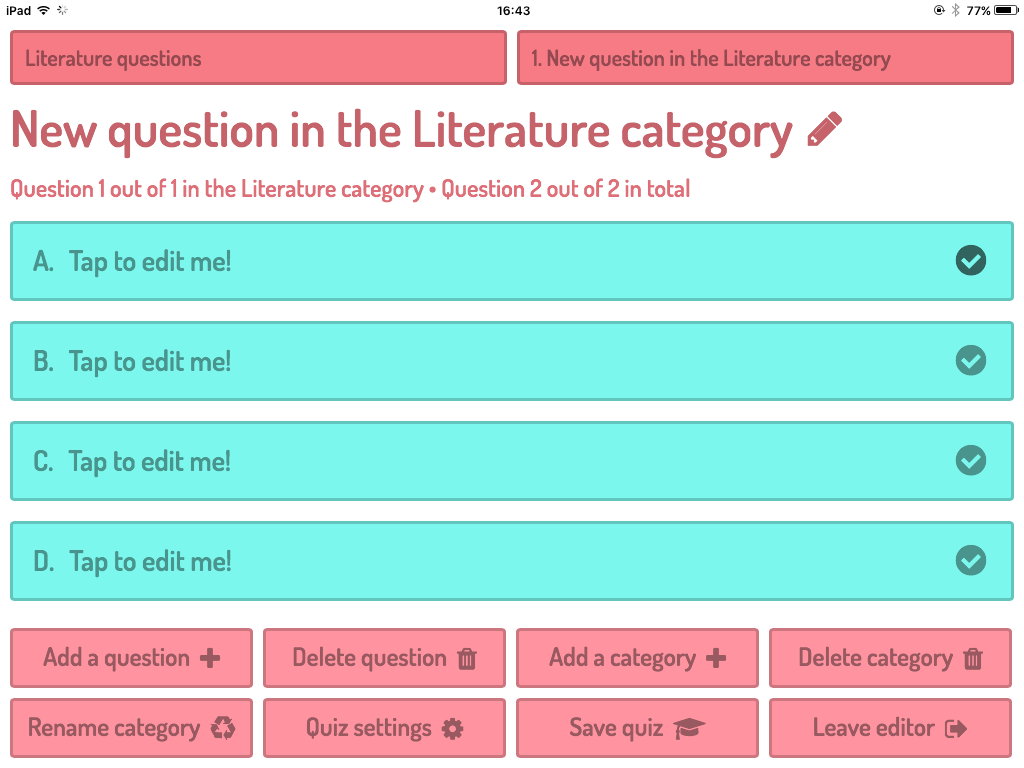
\includegraphics[width=0.95\linewidth]{testing/create_quiz/add_category/after}
  \caption{After}
  \label{fig:sub2}
\end{subfigure}
\caption{Adding a category to the quiz.}
\label{fig:test}
\end{figure}
As expected, a dialog to enter a category name is shown when the add category button is pressed, and the new category is added successfully. \textit{Success.}
% subsubsection add_category (end)


\subsubsection{Delete Category} % (fold)
\label{ssub:add_category}
This ensures that the user is able to succesfully delete their custom categories in the current quiz.
\begin{figure}[!htbp]
\centering
\begin{subfigure}{0.5\textwidth}
  \centering
  \includegraphics[width=0.95\linewidth]{testing/create_quiz/delete_category/before}
  \caption{Before}
  \label{fig:sub1}
\end{subfigure}%
\begin{subfigure}{0.5\textwidth}
  \centering
  \includegraphics[width=0.95\linewidth]{testing/create_quiz/delete_category/after}
  \caption{After}
  \label{fig:sub2}
\end{subfigure}
\caption{Deleting a category from the quiz.}
\label{fig:test}
\end{figure}
As expected, a dialog to enter a category name is shown when the add category button is pressed, and the new category is added successfully. \textit{Success.}
% subsubsection add_category (end)


\subsubsection{Rename Category} % (fold)
\label{ssub:add_category}
This ensures that the user is able to succesfully rename their custom categories in the current quiz.
\begin{figure}[!htbp]
\centering
\begin{subfigure}{0.5\textwidth}
  \centering
  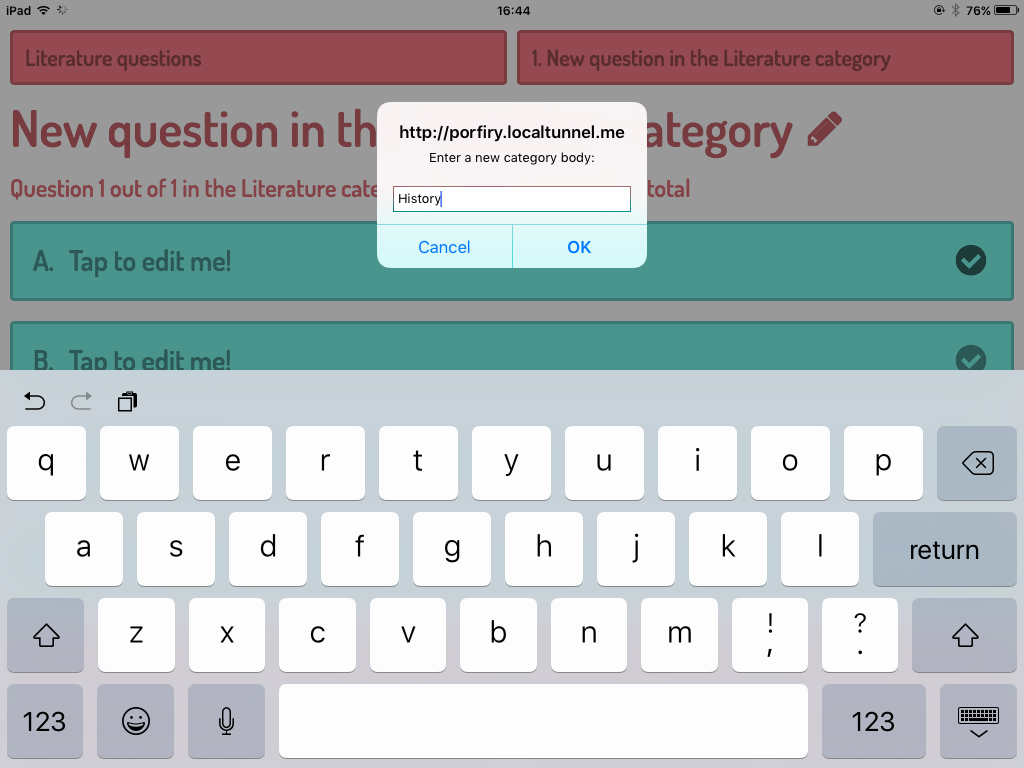
\includegraphics[width=0.95\linewidth]{testing/create_quiz/rename_category/during}
  \caption{During}
  \label{fig:sub1}
\end{subfigure}%
\begin{subfigure}{0.5\textwidth}
  \centering
  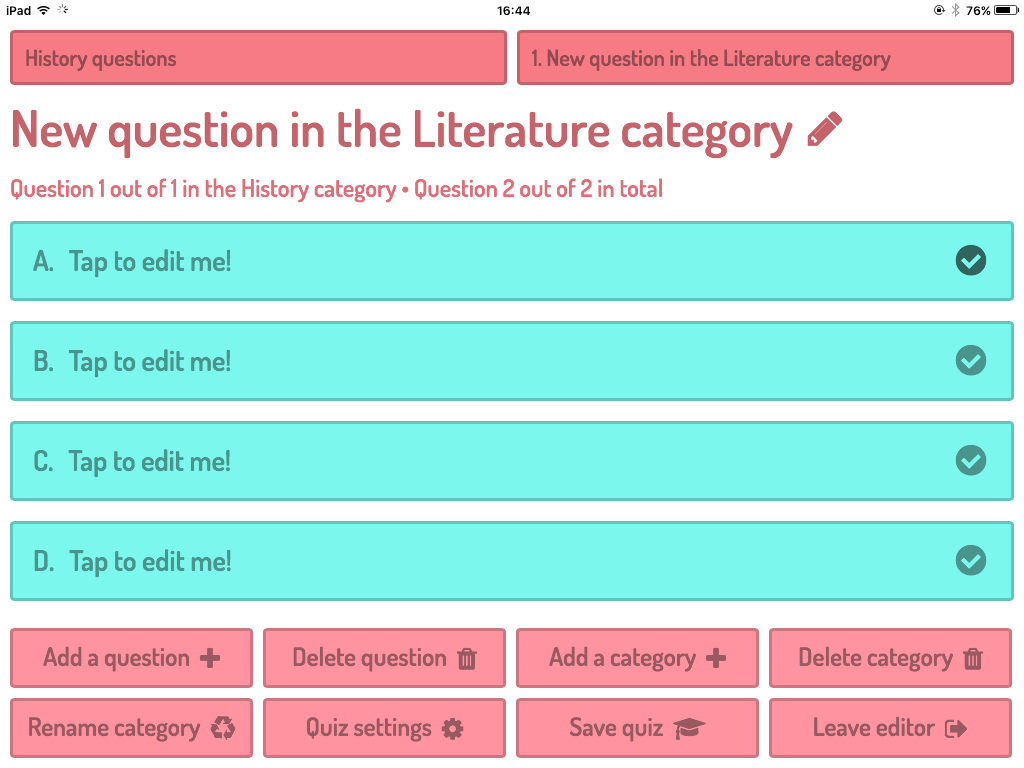
\includegraphics[width=0.95\linewidth]{testing/create_quiz/rename_category/after}
  \caption{After}
  \label{fig:sub2}
\end{subfigure}
\caption{Renaming a category in the quiz.}
\label{fig:test}
\end{figure}
As expected, a dialog to enter the new category name is shown when the rename category button is pressed, and category is renamed successfully. \textit{Success.}
% subsubsection add_category (end)

\subsubsection{Edit Answer} % (fold)
\label{ssub:add_category}
This test ensures that the user is able to edit the body of an answer in the current quiz.
\begin{figure}[!htbp]
\centering
\begin{subfigure}{0.5\textwidth}
  \centering
  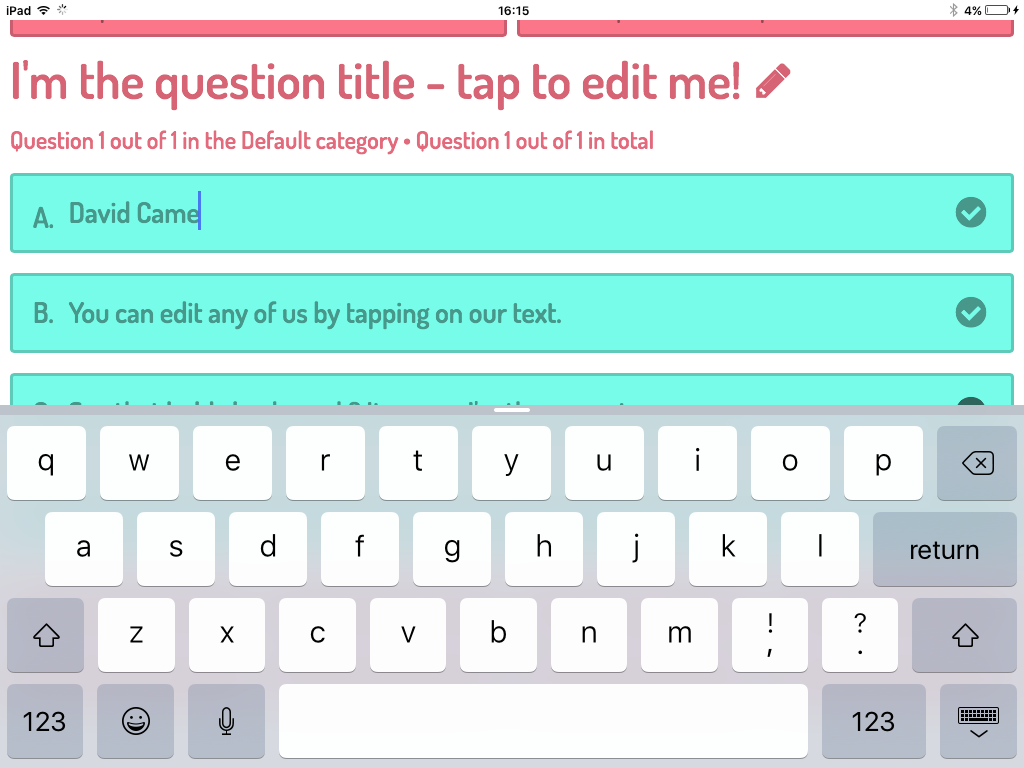
\includegraphics[width=0.95\linewidth]{testing/create_quiz/edit_answer/during}
  \caption{During}
  \label{fig:sub1}
\end{subfigure}%
\begin{subfigure}{0.5\textwidth}
  \centering
  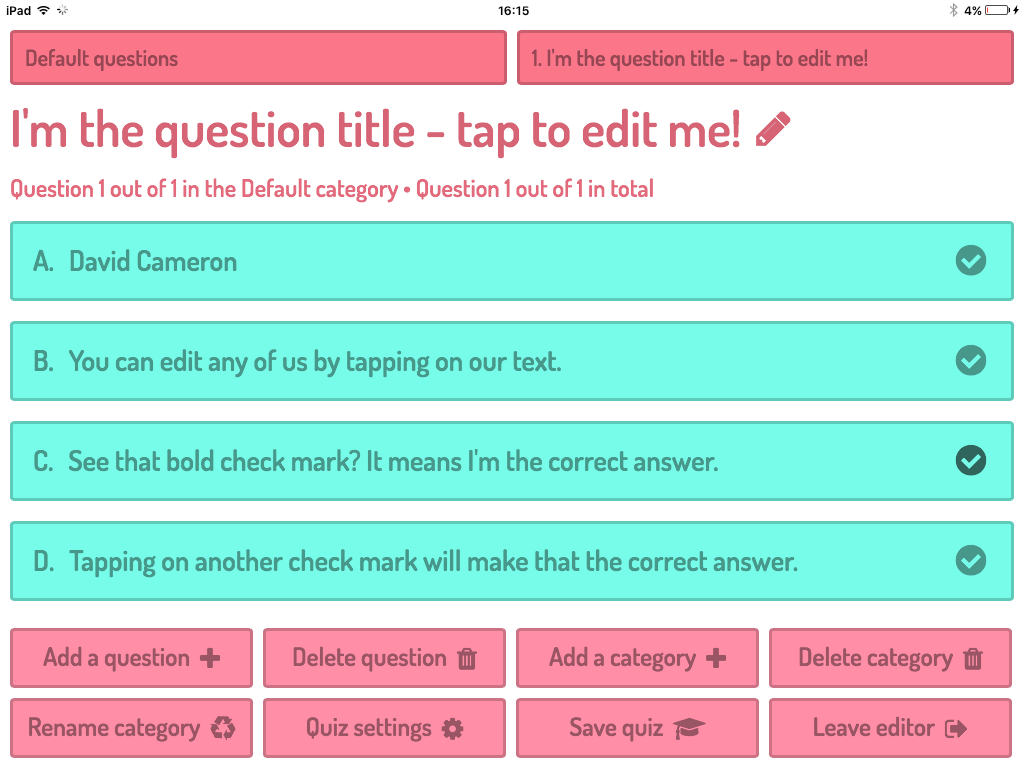
\includegraphics[width=0.95\linewidth]{testing/create_quiz/edit_answer/after}
  \caption{After}
  \label{fig:sub2}
\end{subfigure}
\caption{Marking an answer in as correct.}
\label{fig:test}
\end{figure}
\\As expected, the application allowed for the answer body to be edited, and then persisted this change after leaving the edit mode. \textit{Success.}
% subsubsection add_category (end)


\subsubsection{Mark Answer as Correct} % (fold)
\label{ssub:add_category}
This ensures that the user is able to succesfully mark an answer as correct in the current quiz.
\begin{figure}[!htbp]
\centering
\begin{subfigure}{0.5\textwidth}
  \centering
  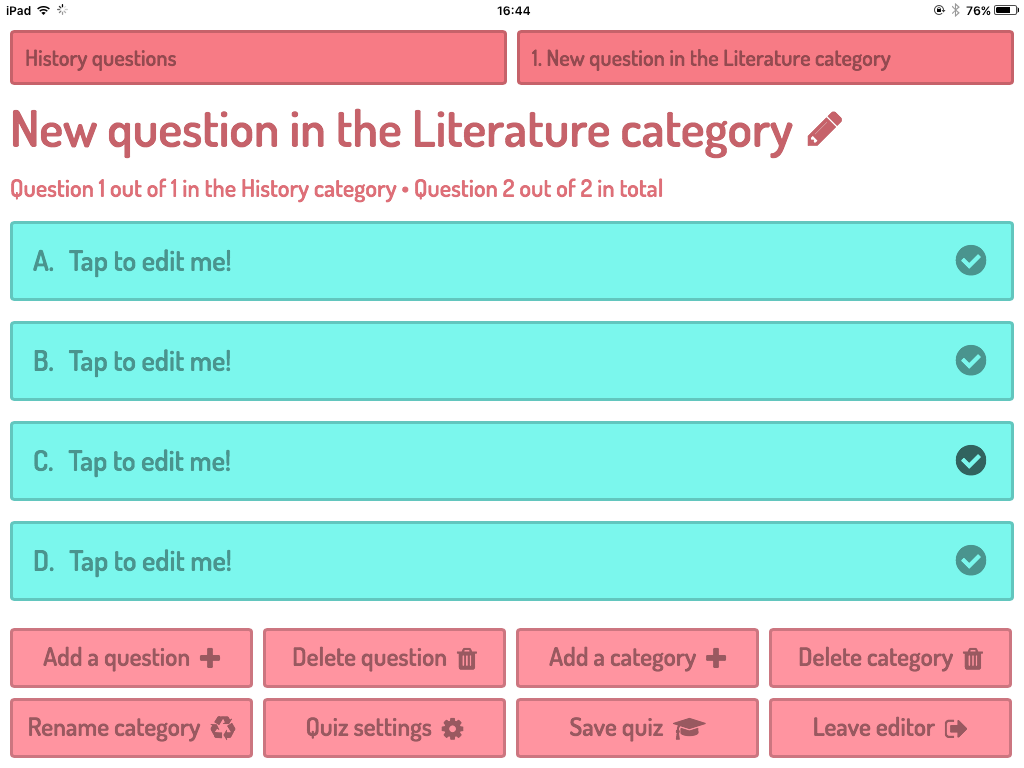
\includegraphics[width=0.95\linewidth]{testing/create_quiz/change_answer/before}
  \caption{During}
  \label{fig:sub1}
\end{subfigure}%
\begin{subfigure}{0.5\textwidth}
  \centering
  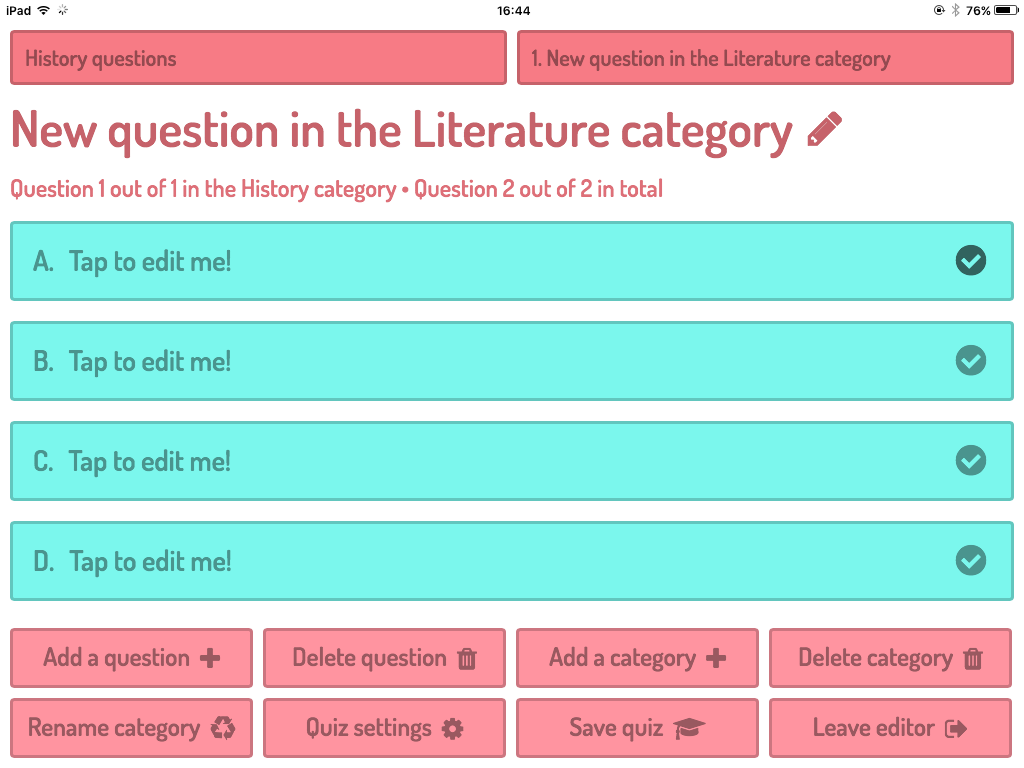
\includegraphics[width=0.95\linewidth]{testing/create_quiz/change_answer/after}
  \caption{After}
  \label{fig:sub2}
\end{subfigure}
\caption{Marking an answer in as correct.}
\label{fig:test}
\end{figure}
\\As expected, the correct mark moved from the third to the first question, meaning that it was marked as correct. \textit{Success.}
% subsubsection add_category (end)


\subsubsection{Save Quiz} % (fold)
\label{ssub:add_category}
This test ensures that the user is able to save their quizzes to the database.
\begin{figure}[!htbp]
\centering
\begin{subfigure}{0.5\textwidth}
  \centering
  \includegraphics[width=0.95\linewidth]{testing/create_quiz/save_quiz/before}
  \caption{During}
  \label{fig:sub1}
\end{subfigure}%
\begin{subfigure}{0.5\textwidth}
  \centering
  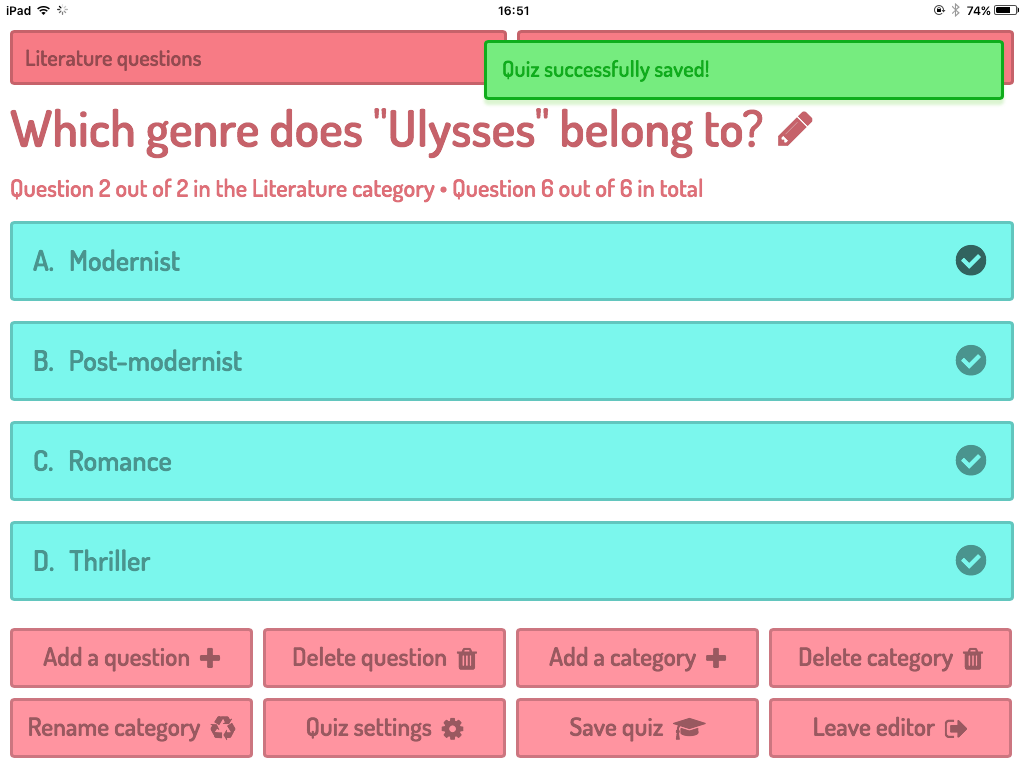
\includegraphics[width=0.95\linewidth]{testing/create_quiz/save_quiz/after}
  \caption{After}
  \label{fig:sub2}
\end{subfigure}
\caption{Saving a quiz to the database.}
\label{fig:test}
\end{figure}
\\As expected, the correct mark moved from the third to the first question, meaning that it was marked as correct. \textit{Success.}
% subsubsection add_category (end)

\subsubsection{Move Questions on Time}
This test ensures that the quiz moves to the correct questions at the correct time, using the test quiz specified in the test plan. Due to the difficulty of taking valid screenshots of this process, a table is included below with room for a teacher to sign as confirmation that this functionality is working.

\begin{table}[]
\centering
\begin{tabular}{|l|l|l|}
\hline
\multicolumn{1}{|c|}{\textbf{Expected result}}              & \multicolumn{1}{c|}{\textbf{Works}} & \multicolumn{1}{c|}{\textbf{Signature}} \\ \hline
Displays "Who is the French Premier?" at 0-10 seconds       & Yes                                 &                                         \\ \hline
Displays "Who won the 1960 World Cup?" at 10-20 seconds     & Yes                                 &                                         \\ \hline
Displays "What is the capital of Iceland?" at 20-30 seconds & Yes                                 &                                         \\ \hline
\end{tabular}
\caption{My caption}
\label{my-label}
\end{table}

\\As can be witnessed, the quiz moves to the correct questions at the correct time, meaning that the test has passed. \texit{Success.}

\subsection{Login Screen Testing} % (fold)
\label{sub:login_screen_testing}
This subsection states how to test that the system themes itself correctly for each house.
% subsection login_screen_testing (end)

\subsubsection{Display Acton Colours} % (fold)
\label{ssub:display_acton_colours}
\begin{enumerate}[leftmargin=*]
\item Select ``Acton'' in the house box.\\\\
\textit{Expected result}: Interface should turn blue.
\end{enumerate}
% subsubsection display_acton_colours (end)

\subsubsection{Display Baxter Colours} % (fold)
\label{ssub:display_baxter_colours}
\begin{enumerate}[leftmargin=*]
\item Select ``Baxter'' in the house box.\\\\
\textit{Expected result}: Interface should turn orange.
\end{enumerate}
% subsubsection display_baxter_colours (end)

\subsubsection{Display Clive Colours} % (fold)
\label{ssub:display_clive_colours}
\begin{enumerate}[leftmargin=*]
\item Select ``Clive'' in the house box.\\\\
\textit{Expected result}: Interface should turn green.
\end{enumerate}
% subsubsection display_clive_colours (end)

\subsubsection{Display Darwin Colours} % (fold)
\label{ssub:display_darwin_colours}
\begin{enumerate}[leftmargin=*]
\item Select ``Darwin'' in the house box.\\\\
\textit{Expected result}: Interface should turn purple.
\end{enumerate}
% subsubsection display_darwin_colours (end)

\subsubsection{Display Houseman Colours} % (fold)
\label{ssub:display_houseman_colours}
\begin{enumerate}[leftmargin=*]
\item Select ``Houseman'' in the house box.\\\\
\textit{Expected result}: Interface should turn red.
\end{enumerate}
% subsubsection display_houseman_colours (end)

\subsubsection{Display Webb Colours} % (fold)
\label{ssub:display_webb_colours}
\begin{enumerate}[leftmargin=*]
\item Select ``Webb'' in the house box.\\\\
\textit{Expected result}: Interface should turn yellow.
\end{enumerate}
% subsubsection display_webb_colours (end)

\subsection{Results Test Runs} % (fold)
\label{sub:results_test_runs}
This section tests that the results screen works correctly.

\subsubsection{Connects to State Store} % (fold)
\label{ssub:connects_to_state_store}
This test ensures that the component can connect to the state store.
% subsubsection connects_to_state_store (end)

\subsubsection{Display Correct Results} % (fold)
\label{ssub:display_correct_results}
This test ensures that the results screen shows the correct results.
% subsubsection display_correct_results (end)
% subsection results_test_runs (end)
\subsection{API Test Runs}
These are the tests for the restful API. The API acts as a means of communicating with the database. In order to do so, certain requests - either GET, POST, PUT or DELETE - are sent to an address; in this case, \textit{/api/quizzes}. The API then looks at the request type that was sent, along with any other data that came with it, and performs the appropriate operation, be that showing a list of all quizzes, showing a specific quiz, or updating a quiz.

\subsubsection{api.spec.js} % (fold)
\label{ssub:api_spec_js}
\lstinputlisting[language=javascript, caption=Unit tests for the API.]{../test/api.spec.js}
\begin{figure}[h!]
  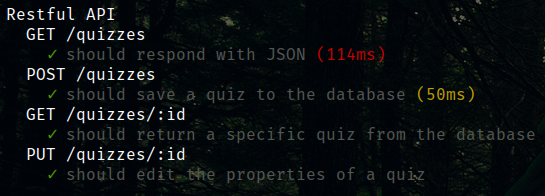
\includegraphics[scale=0.55]{testing/api/api}
  \caption{Test outcome for api.spec.js 1}
\end{figure}
% subsubsection api_spec_js (end)

As can be seen by the little green ticks, all the different HTTP methods passed, proving that the API is working correctly, and thereby allowing requests to be sent from throughout the application. \textit{Success.}



% part testing_ (end)

\section{Acceptance Testing}
The system was passed to a friend for testing, with the request that he note down sections that he both liked and disliked. He had the following positive comments about the application:

\begin{itemize}
  \item The different colour schemes are effective, and are a useful differentiator between the houses. They also give the program a nice, fun feel, which fits in with the audience.

  \item It's very easy to make a quiz, as all the buttons are clear, with all the functions labelled. I think it would be suitable for someone who isn't very skilled with technology.

  \item I really like the bouncing animation on the login screen.

  \item The timer in the play quiz screen makes it really exciting to play on; there's a lot of tension.
\end{itemize}

He also had the following, less positive, notes:

\begin{itemize}
  \item At first I didn't know how to change the question title. You could make this a bit clearer by adding a box around it, or something.

  \item When there are a lot of people on the quiz, the program slows down quite a lot, and the timer bar is very jittery.

  \item It's a shame that there aren't any live visualisations to see what other people are answering.
\end{itemize}

As can be gleaned from the notes above, the tester's overall opinion of the system was strong, especially in the quiz creator interface. This is not surprising, as a large amount of time was spent making this work properly. The quiz playing interface lacks the same amount of polish, and this was picked up by the tester, though he did comment that it was sufficiently tence and exciting due to the inclusion of the live countdown timer.


% 1. Evaluation of test results
% 2. Evaluate against original objectives.
% 3. Evaluate against evaluation criteria.
% 4. Potential future improvements.
\clearpage
\part{Evaluation} % (fold)
\label{prt:evaluation_}
This section contains an extensive evaluation of different parts of the application, and the processes that went into its development. A number of areas have been evaluated, including the test results. In order to qualify the testing process as acceptable, it must be evaluated to ensure that the majority of the testing was successfull; focus will be placed on each of the individual areas of testing that were performed, namely: the unit tests for each individual component, the acceptance testing, and the full system testing. By evaluating all these areas, it will be possible to say whether the test strategy laid out was a success, and the degree to which this is true.

Also evaluated is whether the system meets the original objectives, those objectives outlined at the beginning of the project, before development began, and that took into account the research performed in the analysis section. For the system to considered a success, it must meet all or most of these objectives; this section of the evaluation attempts to determine whether or not this is the case.

The evaluation will also take into account the evaluation criteria - these criteria are additional to the original objectives, and lay out several supplementary aspects that the system should meet to be viewed in a wholly positive light; it also takes into account areas like the length of time spent on actually developing the system. This section of the evaluation therefore evaluations these critera.

Potential future improvements will also be explored. As with any system, there are aspects of it that could be improved. This section outlines several of these, taking into account whether or not they are feasable, and gives methods that could be used to implement them within a reasonable time frame.
% part evaluation_ (end)
\clearpage

\part{User Documentation} % (fold)
\label{prt:user_ _documentation_}
This section outlines how to install and make use of the application.

\section{Installation} % (fold)
\label{sec:installation}
This section details how to install the application. The process is rather specialised, and te precise details vary depending on which cloud provider is being used to host the system, but by and large there is a process that can be followed.
% section installation (end)

\section{Usage} % (fold)
\label{sec:usage}
This section displays how to use the quiz system for it's intended purpose. The different parts of the system have been split up into different subsections for convenience.

\subsection{Creating a New Quiz} % (fold)
\label{sub:creating_a_quiz}
Creating a new quiz is a very simple process. Select your house and year from the drop down lists on the menu, and then press the ``Create a new quiz'' button.
% subsection creating_a_quiz (end)

\subsection{Editing a Quiz} % (fold)
\label{sub:editing_a_quiz}
The interface for adding questions and answers to a quiz is similar to other quiz creation systems you may have used in the past. When a quiz is first created, there is one question, with four answers - all of these can be edited.

\subsubsection{Editing a Question} % (fold)
\label{ssub:editing_a_question}
To edit a question's title, simply click or tap the current title, and type in your changes.
% subsubsection editing_a_question (end)

\subsubsection{Editing an Answer} % (fold)
\label{ssub:editing_an_answer}
To edit a question's answer, simply click or tap the current answer, and type in your changes.
% subsubsection editing_an_answer (end)

\subsubsection{Marking an Answer as Correct} % (fold)
\label{ssub:marking_an_answer_as_correct}
To mark an answer as correct, tap the tick icon at the end of the answer. The answer currently marked as correct will no longer be so.
% subsubsection marking_an_answer_as_correct (end)

\subsubsection{Adding a Question} % (fold)
\label{ssub:adding_a_question}
To add a new question, simply press the ``Add Question'' button.
% subsubsection adding_a_question (end)

% subsection editing_a_quiz (end)

\subsection{Scheduling a Quiz} % (fold)
\label{sub:scheduling_a_quiz}

% subsection scheduling_a_quiz (end)

\subsection{Loading a Quiz} % (fold)
\label{sub:loading_a_quiz}
If you wish to load a quiz that has been created earlier, for further editing, press the ``Load quiz'' button on the main menu, and locate the quiz you wish to edit by its title and schedule date. From there, press the ``Edit quiz'' button, and you will be taken to the familiar quiz editing interface.
% subsection loading_a_quiz (end)

\subsection{Deleting a Quiz} % (fold)
\label{sub:deleting_a_quiz}
Deleting a quiz is also very simple. Press the ``Load quiz'' button on the main menu, and locate the quiz you wish to edit by its title and schedule date. From there, press the ``Delete quiz'' button, and the quiz will be deleted. \textit{\textbf{Note:} if the quiz has been scheduled to play, deleting the quiz will cancel this schedule, and the quiz will no longer take place.}
% subsection deleting_a_quiz (end)
% section usage (end)
% part user_ _documentation_ (end)

\end{document}
